\documentclass[a4paper]{report}
\usepackage[utf8]{inputenc}
\usepackage{amsmath,amssymb,amsfonts,amsthm,stmaryrd}
\usepackage{mathrsfs} % per mathscr
\usepackage{dsfont} % per mathbb1
\usepackage{graphicx}% ruota freccia per le azioni
\usepackage{oldgerm} % Fractur Particolare
\usepackage{marvosym}% per il \Lightning
\usepackage{array}
\usepackage{faktor} %per gli insiemi quoziente
\usepackage{hyperref}
\usepackage{xparse} % Per nuovi comandi con tanti input opzionali
\usepackage{tikz-cd}
\usepackage{multicol}
\usepackage{multirow}
\usepackage{cancel}

%\usepackage[italian]{babel}
\usepackage[position=top]{subfig}
\usepackage{setspace}
\usepackage{mdframed}
\usepackage{calc}
\usepackage{enumerate}
\usepackage{centernot}
\usepackage{comment}

\usepackage{ mathdots }

% Ambienti per teoremi =================================
% <name> 
% <space above> 
% <space below> 
% <body font> 
% <indent amount> 
% <Theorem head font> 
% <punctuation after theorem head> 
% <space after theorem head> (default .5em) 
% <Theorem head spec>

% I nuovi ambienti sono costruiti in modo da andare alla riga successiva

\newsavebox{\boiteencadrement}
\newenvironment{encadrement}[1][gray!15]
  {\par\addvspace{\topsep+10pt}%
   \def\couleurencadrement{#1}%
   \begin{lrbox}{\boiteencadrement}%
   \begin{minipage}{\linewidth-6\fboxsep-1pt}%
  }
  {\end{minipage}\end{lrbox}%
   \noindent
\begin{tikzpicture}[
   inner sep=8pt,
   line width=0.75pt]
   \node[rounded corners = 5pt,
   draw,
   color=black,
   fill=\couleurencadrement] {\usebox{\boiteencadrement}};
   \end{tikzpicture}%
   \par\addvspace{\topsep+10pt}%
  }

%Equazioni
\numberwithin{equation}{section} 

%Teoremi
\theoremstyle{plain}

%\newtheorem{lem}[thm]{Lemma}
%\newtheorem{exer}[thm]{Esercizio}
%\newtheorem{cor}[thm]{Corollary}

\theoremstyle{definition}

\newcounter{theorem}
\counterwithin{theorem}{chapter}

    %thm
\newtheorem{pretrm}[theorem]{Theorem}
\newenvironment{theorem}{\begin{encadrement}\begin{pretrm}}{\end{pretrm}\end{encadrement}}

\newtheorem{prefct}[theorem]{Fact}
\newenvironment{fact}{\begin{encadrement}\begin{prefct}}{\end{prefct}\end{encadrement}}

%\newtheorem{definition}[theorem]{Definition}
%\newcounter{definition}
    %def
\newtheorem{predef}[theorem]{Definition}
\newenvironment{definition}{\begin{encadrement}\begin{predef}}{\end{predef}\end{encadrement}}
    %prop
\newtheorem{preprop}[theorem]{Proposition}
\newenvironment{proposition}{\begin{encadrement}\begin{preprop}}{\end{preprop}\end{encadrement}}
    %cor
\newtheorem{precor}[theorem]{Corollary}
\newenvironment{corollary}{\begin{encadrement}\begin{precor}}
{\end{precor}\end{encadrement}}
    %lem
\newtheorem{prelem}[theorem]{Lemma}
\newenvironment{lemma}{\begin{encadrement}\begin{prelem}}{\end{prelem}\end{encadrement}}
%
\newtheorem{conjecture}[theorem]{Conjecture}
\newtheorem{example}[theorem]{Example}
\newtheorem{exercise}[theorem]{Exercise}
\newtheorem{remark}[theorem]{Remark}
\newtheorem*{notation}{Notation}

\makeatletter
\renewenvironment{proof}[1][\proofname]
{
    \par
    \pushQED{\qed}
    \normalfont \topsep6\p@\@plus6\p@\relax
    \trivlist
    \item[\hskip\labelsep\itshape#1\@addpunct{.}]\mbox{}\\*
}
{
    \popQED\endtrivlist\@endpefalse
}
\makeatother



%========= Preambolo per quiver ================
% quiver e' uno strumento che uso spesso per
% disegnare diagrammi. L'interfaccia sul loro sito
% permette di creare in modo visivo il diagramma e
% poi esportarlo come codice LaTeX da inserire nel
% documento. Il sito e' https://q.uiver.app/ 

%-----------------------------------------------
% *** quiver ***
% A package for drawing commutative diagrams exported from https://q.uiver.app.
%
% This package is currently a wrapper around the `tikz-cd` package, importing necessary TikZ
% libraries, and defining a new TikZ style for curves of a fixed height.
%
% Version: 1.2.1
% Authors:
% - varkor (https://github.com/varkor)
% - Andr\e'C (https://tex.stackexchange.com/users/138900/andr%C3%A9c)

\NeedsTeXFormat{LaTeX2e}
%\ProvidesPackage{quiver}[2021/01/11 quiver]

% `tikz-cd` is necessary to draw commutative diagrams.
\RequirePackage{tikz-cd}
% `amssymb` is necessary for `\lrcorner` and `\ulcorner`.
\RequirePackage{amssymb}
% `calc` is necessary to draw curved arrows.
\usetikzlibrary{calc}
% `pathmorphing` is necessary to draw squiggly arrows.
\usetikzlibrary{decorations.pathmorphing}

% A TikZ style for curved arrows of a fixed height, due to Andr\e'C.
\tikzset{curve/.style={settings={#1},to path={(\tikztostart)
    .. controls ($(\tikztostart)!\pv{pos}!(\tikztotarget)!\pv{height}!270:(\tikztotarget)$)
    and ($(\tikztostart)!1-\pv{pos}!(\tikztotarget)!\pv{height}!270:(\tikztotarget)$)
    .. (\tikztotarget)\tikztonodes}},
    settings/.code={\tikzset{quiver/.cd,#1}
        \def\pv##1{\pgfkeysvalueof{/tikz/quiver/##1}}},
    quiver/.cd,pos/.initial=0.35,height/.initial=0}

% TikZ arrowhead/tail styles.
\tikzset{tail reversed/.code={\pgfsetarrowsstart{tikzcd to}}}
\tikzset{2tail/.code={\pgfsetarrowsstart{Implies[reversed]}}}
\tikzset{2tail reversed/.code={\pgfsetarrowsstart{Implies}}}
% TikZ arrow styles.
\tikzset{no body/.style={/tikz/dash pattern=on 0 off 1mm}}
%=================================================

%PER CAMBIARE I MARGINI
\usepackage[margin=4cm]{geometry}

%\usepackage{emptypage} % Pagine vuote non numerate
%\usepackage{fancyhdr} % Sistema headers
%\usepackage[Lenny]{fncychap} % Capitoli fighi
%\ChTitleVar{\Huge\bfseries}
\usepackage[hang,flushmargin]{footmisc} % Footnote non indentata


%========== Stile header e footer ==============

%\pagestyle{fancy}
% Left, Right, Even(pages), Odd(pages), Center
%\fancyhead[L]{\leftmark}
%\fancyfoot[C]{}

%\renewcommand{\chaptermark}[1]{\markboth{\textsc{#1}}{}}
%\renewcommand{\sectionmark}[1]{\markright{\textsc{#1}}}

%\renewcommand{\headrulewidth}{0.05pt}
%\renewcommand{\footnoterule}{\kern 0pt	\hrule width \textwidth height 0.5pt \kern 5pt}

%Numeri pagina in prima pagina capitoli
%\makeatletter
%\let\ps@plain\ps@empty
%\makeatother

%==== Colore dei footnote, link e citazioni ====
\definecolor{DarkBlue}{HTML}{00518B}
\definecolor{DarkRed}{HTML}{B6321C}
\hypersetup{
    colorlinks=true,
    linkcolor=DarkRed,
    filecolor=blue,
    citecolor = DarkRed,
    urlcolor=cyan,
}
\renewcommand\thefootnote{\textcolor{blue}{\arabic{footnote}}}
%============ Simboli standard =================
%----------------- Lettere ---------------------
\newcommand{\A}{\mathbb{A}}
\newcommand{\B}{\mathbb{B}}
\newcommand{\C}{\mathbb{C}}
\newcommand{\D}{\mathbb{D}}
\newcommand{\E}{\mathbb{E}}
\newcommand{\F}{\mathbb{F}}
\newcommand{\G}{\mathbb{G}}
\newcommand{\Hb}{\mathbb{H}}
\newcommand{\I}{\mathbb{I}}
\newcommand{\J}{\mathbb{J}}
\newcommand{\K}{\mathbb{K}}
\newcommand{\Lb}{\mathbb{L}}
\newcommand{\M}{\mathbb{M}}
\newcommand{\N}{\mathbb{N}}
\newcommand{\Ob}{\mathbb{O}}
\newcommand{\Pj}{\mathbb{P}}
\newcommand{\Q}{\mathbb{Q}}
\newcommand{\R}{\mathbb{R}}
\newcommand{\Sb}{\mathbb{S}}
\newcommand{\T}{\mathbb{T}}
\newcommand{\U}{\mathbb{U}}
\newcommand{\V}{\mathbb{V}}
\newcommand{\W}{\mathbb{W}}
\newcommand{\X}{\mathbb{X}}
\newcommand{\Y}{\mathbb{Y}}
\newcommand{\Z}{\mathbb{Z}}

\newcommand{\Ac}{\mathcal{A}}
\newcommand{\Bc}{\mathcal{B}}
\newcommand{\Cc}{\mathcal{C}}
\newcommand{\Dc}{\mathcal{D}}
\newcommand{\Ec}{\mathcal{E}}
\newcommand{\Fc}{\mathcal{F}}
\newcommand{\Gc}{\mathcal{G}}
\newcommand{\Hc}{\mathcal{H}}
\newcommand{\Ic}{\mathcal{I}}
\newcommand{\Jc}{\mathcal{J}}
\newcommand{\Kc}{\mathcal{K}}
\newcommand{\Lc}{\mathcal{L}}
\newcommand{\Mc}{\mathcal{M}}
\newcommand{\Nc}{\mathcal{N}}
\newcommand{\Oc}{\mathcal{O}}
\newcommand{\Pc}{\mathcal{P}}
\newcommand{\Qc}{\mathcal{Q}}
\newcommand{\Rc}{\mathcal{R}}
\newcommand{\Sc}{\mathcal{S}}
\newcommand{\Tc}{\mathcal{T}}
\newcommand{\Uc}{\mathcal{U}}
\newcommand{\Vc}{\mathcal{V}}
\newcommand{\Wc}{\mathcal{W}}
\newcommand{\Xc}{\mathcal{X}}
\newcommand{\Yc}{\mathcal{Y}}
\newcommand{\Zc}{\mathcal{Z}}

\newcommand{\Af}{\mathfrak{A}}
\newcommand{\Bf}{\mathfrak{B}}
\newcommand{\Cf}{\mathfrak{C}}
\newcommand{\Df}{\mathfrak{D}}
\newcommand{\Ef}{\mathfrak{E}}
\newcommand{\Ff}{\mathfrak{F}}
\newcommand{\Gf}{\mathfrak{G}}
\newcommand{\Hf}{\mathfrak{H}}
\newcommand{\If}{\mathfrak{I}}
\newcommand{\Jf}{\mathfrak{J}}
\newcommand{\Kf}{\mathfrak{K}}
\newcommand{\Lf}{\mathfrak{L}}
\newcommand{\Mf}{\mathfrak{M}}
\newcommand{\Nf}{\mathfrak{N}}
\newcommand{\Of}{\mathfrak{O}}
\newcommand{\Pf}{\mathfrak{P}}
\newcommand{\Qf}{\mathfrak{Q}}
\newcommand{\Rf}{\mathfrak{R}}
\newcommand{\Sf}{\mathfrak{S}}
\newcommand{\Tf}{\mathfrak{T}}
\newcommand{\Uf}{\mathfrak{U}}
\newcommand{\Vf}{\mathfrak{V}}
\newcommand{\Wf}{\mathfrak{W}}
\newcommand{\Xf}{\mathfrak{X}}
\newcommand{\Yf}{\mathfrak{Y}}
\newcommand{\Zf}{\mathfrak{Z}}

\newcommand{\af}{\mathfrak{a}}

\newcommand{\cf}{\mathfrak{c}}
\newcommand{\df}{\mathfrak{d}}
\newcommand{\ef}{\mathfrak{e}}
\newcommand{\ff}{\mathfrak{f}}
\newcommand{\gf}{\mathfrak{g}}
\newcommand{\hf}{\mathfrak{h}}

\newcommand{\jf}{\mathfrak{j}}
\newcommand{\kf}{\mathfrak{k}}
\newcommand{\lf}{\mathfrak{l}}
\newcommand{\mf}{\mathfrak{m}}
\newcommand{\nf}{\mathfrak{n}}
\newcommand{\of}{\mathfrak{o}}
\newcommand{\pf}{\mathfrak{p}}
\newcommand{\qf}{\mathfrak{q}}
\newcommand{\rf}{\mathfrak{r}}

\newcommand{\tf}{\mathfrak{t}}
\newcommand{\uf}{\mathfrak{u}}
\newcommand{\vf}{\mathfrak{v}}
\newcommand{\wf}{\mathfrak{w}}
\newcommand{\xf}{\mathfrak{x}}
\newcommand{\yf}{\mathfrak{y}}
\newcommand{\zf}{\mathfrak{z}}

\newcommand{\As}{\mathscr{A}}
\newcommand{\Bs}{\mathscr{B}}
\newcommand{\Cs}{\mathscr{C}}
\newcommand{\Ds}{\mathscr{D}}
\newcommand{\Es}{\mathscr{E}}
\newcommand{\Fs}{\mathscr{F}}
\newcommand{\Gs}{\mathscr{G}}
\newcommand{\Hs}{\mathscr{H}}
\newcommand{\Is}{\mathscr{I}}
\newcommand{\Js}{\mathscr{J}}
\newcommand{\Ks}{\mathscr{K}}
\newcommand{\Ls}{\mathscr{L}}
\newcommand{\Ms}{\mathscr{M}}
\newcommand{\Ns}{\mathscr{N}}
\newcommand{\Os}{\mathscr{O}}
\newcommand{\Ps}{\mathscr{P}}
\newcommand{\Qs}{\mathscr{Q}}
\newcommand{\Rs}{\mathscr{R}}
\newcommand{\Ss}{\mathscr{S}}
\newcommand{\Ts}{\mathscr{T}}
\newcommand{\Us}{\mathscr{U}}
\newcommand{\Vs}{\mathscr{V}}
\newcommand{\Ws}{\mathscr{W}}
\newcommand{\Xs}{\mathscr{X}}
\newcommand{\Ys}{\mathscr{Y}}
\newcommand{\Zs}{\mathscr{Z}}

\newcommand{\ula}{{\underline{a}}}
\newcommand{\ulb}{{\underline{b}}}
\newcommand{\ulc}{{\underline{c}}}
\newcommand{\uld}{{\underline{d}}}
\newcommand{\ule}{{\underline{e}}}
\newcommand{\ulf}{{\underline{f}}}
\newcommand{\ulg}{{\underline{g}}}
\newcommand{\ulh}{{\underline{h}}}
\newcommand{\uli}{{\underline{i}}}
\newcommand{\ulj}{{\underline{j}}}
\newcommand{\ulk}{{\underline{k}}}
\newcommand{\ull}{{\underline{l}}}
\newcommand{\ulm}{{\underline{m}}}
\newcommand{\uln}{{\underline{n}}}
\newcommand{\ulo}{{\underline{o}}}
\newcommand{\ulp}{{\underline{p}}}
\newcommand{\ulq}{{\underline{q}}}
\newcommand{\ulr}{{\underline{r}}}
\newcommand{\uls}{{\underline{s}}}
\newcommand{\ult}{{\underline{t}}}
\newcommand{\ulu}{{\underline{u}}}
\newcommand{\ulv}{{\underline{v}}}
\newcommand{\ulw}{{\underline{w}}}
\newcommand{\ulx}{{\underline{x}}}
\newcommand{\uly}{{\underline{y}}}
\newcommand{\ulz}{{\underline{z}}}

%---------- Funzioni standard ------------------
\DeclareMathOperator{\Adj}{Adj}
\DeclareMathOperator{\adj}{adj}
\DeclareMathOperator{\Ann}{Ann}
\DeclareMathOperator{\Arg}{Arg}
\DeclareMathOperator{\Ass}{Ass}
\DeclareMathOperator{\cha}{char}
\DeclareMathOperator{\cod}{cod}
\DeclareMathOperator{\coker}{coker}
\DeclareMathOperator{\comb}{Comb}
\DeclareMathOperator{\dom}{dom}
\DeclareMathOperator{\End}{End}
\DeclareMathOperator{\Fix}{Fix}
\DeclareMathOperator{\Frac}{Frac}
\DeclareMathOperator{\Hom}{Hom}
\DeclareMathOperator{\imm}{Imm}
\DeclareMathOperator{\Ind}{Ind}
\DeclareMathOperator*{\infess}{infess}
\DeclareMathOperator{\mcd}{mcd}
\DeclareMathOperator{\mcm}{mcm}
\DeclareMathOperator{\Min}{Min}
\DeclareMathOperator{\Mor}{Mor}
\DeclareMathOperator{\obj}{obj}
\DeclareMathOperator{\orb}{orb}
\DeclareMathOperator{\ord}{ord}
\DeclareMathOperator{\Proj}{Proj}
\DeclareMathOperator{\Res}{Res}
\DeclareMathOperator{\rnk}{rnk}
\DeclareMathOperator{\sgn}{sgn}
\DeclareMathOperator{\Span}{Span}
\DeclareMathOperator{\Spec}{Spec}
\DeclareMathOperator{\stab}{stab}
\DeclareMathOperator*{\supess}{supess}
\DeclareMathOperator{\Supp}{Supp}
\DeclareMathOperator{\supp}{supp}
\DeclareMathOperator{\Sym}{Sym}
\DeclareMathOperator{\tr}{tr}

\newcommand{\Real}{\,\Re\mathfrak{e}}
\newcommand{\Imag}{\,\Im\mathfrak{m}}



%-------------- Frecce -------------------------
\newcommand{\coimplies}{\Longleftrightarrow}
\newcommand{\inj}{\hookrightarrow}
\newcommand{\onto}{\twoheadrightarrow}
\newcommand{\ot}{\leftarrow}
\newcommand{\acts}{\curvearrowright}

%----------- Lettere greche -------------------
\newcommand{\al}{\alpha}
\newcommand{\de}{\delta}
\newcommand{\e}{\varepsilon}
%\newcommand{\th}{\theta}
\newcommand{\la}{\lambda}
\newcommand{\vp}{\varphi}

%-------------- Derivate ----------------------
\newcommand{\raiseargument}[1]{\raisebox{.8ex}{$#1$}}
\newcommand{\centersmallmath}[1]{\vcenter{\hbox{\scalebox{.8}{$#1$}}}}
\newcommand{\raiseargumentsmall}[1]{\raisebox{.4ex}{\scalebox{.8}{$#1$}}}
\newcommand*{\emptyfrac}[2]{\genfrac{}{}{0pt}{}{#1}{#2}}

\NewDocumentCommand{\ddxi}{O{x}mm}{
    {\frac{d^{}{#3}}{d{#1}_{#2}}}
}

\NewDocumentCommand{\dd}{O{}mm}{
    {\frac{d^{#1}{#3}}{d{#2}^{#1}}}
}

\NewDocumentCommand{\ppxi}{O{x}mm}{
    {{\frac{\partial^{}{#3}}{\partial{#1}_{#2}}}}
}

\NewDocumentCommand{\pp}{O{}mm}{
    {{\frac{\partial^{#1}{#3}}{\partial{#2}}}}
}





%========== Comandi dattilografici ============
%--------- Passaggi in derivazioni ------------
\newcommand{\pasg}[3]{\overset{\hyperref[#3]{\text{#2}}}{#1}}
\newcommand{\pasgnl}[2]{\overset{\text{#2}}{#1}}
\newcommand{\pasgnlmath}[2]{\overset{#2}{#1}}
\newcommand{\pasgmath}[3]{\overset{\hyperref[#3]{{#2}}}{#1}}

%----------- Modifica testo -------------------
\newcommand{\ul}[1]{\underline{#1}}
\newcommand{\ol}[1]{\overline{#1}}
\newcommand{\wt}[1]{\widetilde{#1}}
\newcommand{\wh}[1]{\widehat{#1}}
\newcommand{\td}[1]{\Tilde{#1}}
\newcommand{\rg}[1]{{\mathring {#1}}}
\newcommand{\under}[2]{\underset{#1}{\underbrace{#2}}}

%-------------- Parentesi ---------------------
\newcommand{\pa}[1]{\left({#1}\right)}
\newcommand{\spa}[1]{\left[{#1}\right]}
\newcommand{\cpa}[1]{\left\{{#1}\right\}}
\newcommand{\abs}[1]{\left|{#1}\right|}
\newcommand{\norm}[1]{\left\Vert{#1}\right\Vert}
\newcommand{\ps}[1]{\left\langle {#1}\right\rangle}
\newcommand{\floor}[1]{\left\lfloor {#1}\right\rfloor}
\newcommand{\ceil}[1]{\left\lceil {#1}\right\rceil}
\newcommand{\rbar}[1]{\left.{#1}\right|}

%--------------- Matrici ----------------------
\newcommand{\mat}[1]{\begin{pmatrix}#1\end{pmatrix}}
\newcommand{\emat}[1]{\begin{matrix}#1\end{matrix}}
\newcommand{\dmat}[1]{\begin{vmatrix}#1\end{vmatrix}}
\newcommand{\smat}[1]{\begin{smallmatrix}#1\end{smallmatrix}}
\newcommand{\BIG}[1]{\mathlarger{\mathlarger{\mathlarger{\mathlarger{#1}}}}}

%--------------- Funzioni ---------------------
\newcommand{\funcDef}[4]{
\begin{array}{ccc}
{#1} & \longrightarrow & {#2}\\
{#3} & \longmapsto & {#4}
\end{array}}
\newcommand{\functorDef}[6]{
\begin{array}{ccc}
{#1} & \longrightarrow & {#2}\\
{#3} & \longmapsto & {#4}\\
{#5} & \longmapsto & {#6}
\end{array}}
\newcommand{\correspDef}[6]{
\begin{array}{ccc}
{#1} & \longleftrightarrow & {#2}\\
{#3} & \longmapsto & {#4}\\
{#5} & \longmapsfrom & {#6}
\end{array}}

%---------------- Altro -----------------------
\newcommand{\bs}{\setminus}
\newcommand{\res}[1]{\raisebox{-.5ex}{$|$}_{#1}}
\newcommand{\quot}[2]{\faktor{#1}{#2}}
\newcommand{\sep}{\,\middle|\,}

\newcommand{\ii}{^{-1}}
\newcommand{\nz}{\bs\{0\}}

\newcommand{\powerset}{\mathscr{P}}
\newcommand{\del}{\partial}
\newcommand{\0}{{\underline{0}}}
\newcommand{\1}{{\vcenter{\hbox{\scalebox{1.2}{$\mathds{1}$}}}}}
\newcommand{\bw}{\bigwedge}


\newcommand{\GL}{\mathrm{GL}}
\newcommand{\PGL}{\mathrm{PGL}}
\newcommand{\SL}{\mathrm{SL}}
%\NewDocumentCommand{\PGL}{o m}{
%    \IfNoValueTF{#1}
%        {{\mathbb{P}GL({#2})}}
%    {{\mathbb{P}GL_{#1}({#2})}}
%}
%\NewDocumentCommand{\GL}{o m}{
%    \IfNoValueTF{#1}
%        {{GL({#2})}}
%    {{GL_{#1}({#2})}}
%}
\newcommand{\znz}[1]{{\Z/{#1}\Z}}







\usepackage{cleveref}


% ============================================


%---------- Comandi specifici ----------------
\DeclareMathOperator{\Der}{Der}
\DeclareMathOperator{\SO}{SO}
\DeclareMathOperator{\Mat}{Mat}
\DeclareMathOperator{\Fun}{Fun}
\DeclareMathOperator{\Conv}{Conv}
\DeclareMathOperator{\Cone}{Cone}
\DeclareMathOperator{\Bl}{Bl}
\DeclareMathOperator{\Relint}{Relint}
\DeclareMathOperator{\Star}{Star}
\DeclareMathOperator{\Ext}{Ext}
\DeclareMathOperator{\Tor}{Tor}
\DeclareMathOperator{\Div}{Div}
\DeclareMathOperator{\CDiv}{CDiv}
\DeclareMathOperator{\Cl}{Cl}
\DeclareMathOperator{\Pic}{Pic}

\newcommand{\Diag}{\mathrm{Diag}}
\newcommand{\Ab}{\mathrm{Ab}}
\newcommand{\Mon}{\mathrm{Mon}}

\newcommand{\op}{^{op}}

%--------- Comandi dattilografici ------------
\newcommand{\coloneqq}{:=}
\renewcommand{\div}{\mathrm{div}}


% ============================================
\title{\huge Toric Varieties - Geometria Algebrica F
\vspace{0.7cm}

\Large Corso del prof. Talpo Mattia}

\author{\Large Francesco Sorce}
\date{Università di Pisa\\
Dipartimento di Matematica\\
A.A. 2024/25}

\begin{document}
\maketitle

%\newpage
\tableofcontents
\newpage

\chapter*{Introduction}
\section*{Syllabus}
The first part of the course deals with:
\begin{itemize}
    \item Algebraic Tori, their actions and representations
    \item Affine toric varieties (with monoids) $\leftrightarrow$ cones in some $\R^n$
    \item Projective toric varieties $\leftrightarrow$ polytopes in some $\R^n$
    \item General toric varieties $\leftrightarrow$ fans in $\R^n$
\end{itemize}
We will then deal with (subject to change)
\begin{itemize}
    \item Divisors/line bundles on toric varieties
    \item Cox ring of a toric variety
    \item Cohomology of divisors
    \item Toric morphisms and resolution of singularities
    \item and more...?
\end{itemize}
The main reference for this course \textemdash ``Toric varieties" by Cox, Little, Schenck \cite{cox2011toric} \textemdash is available in the same folder as this PDF.

\section*{What is the course about?}
We will work over an algebraically closed field (and we will be lax about the characteristic of the field). In \cite{cox2011toric} the authors work over $\C$ but many results hold more generally.
\medskip

The main goal of the course is understanding toric varieties:
\begin{definition}[Toric variety]
An $n$-dimensional toric variety $X$ is a (normal) $k$-variety equipped with an open immersion of an $n$-dimensional torus $T\subseteq X$, where $T\cong (k^\ast)^n$, and an action $T\times T\to T$ which extends to the whole of $X$ \footnote{that is, it extends to a $T\times X\to X$}.
\end{definition}

\begin{remark}
Normality is a standard assumption that we'll make at some point but some things work without it.
\end{remark}

We'll see that the geometry of such an object is encoded in a combinatorial gadget, converting problems in algebraic geometry to problems in combinatorics, which is sometimes convenient.

The opposite reduction is also possible and has been used historically. One of the main examples of a combinatorial problem being solved via the geometry of toric varieties is
\begin{example}[McMullen's ``$g$-conjecture"]

The then conjecture, and now theorem, is a characterization of the $f$-vectors of simple polytopes\footnote{for now a simple polytope is the convex hull of a finite subset of $\R^n$}.

\begin{definition}[$f$-vectors]
If $P$ is a polytope, its \textbf{$f$-vector} is 
\[(f_0(P),\cdots, f_d(P)),\quad \text{where $d=\dim P$}\]
and $f_i(P)$ is the number of $i$-dimensional faces. We may set $f_{-1}(P)=1$.
\end{definition}

It's reasonable to ask ourselves which $f$-vectors can appear. We may define the \textbf{$h$-vector} by setting
\[\sum_{i=0}^d f_i (t-1)^i=\sum_{i=0}^dh_i t^i,\quad \text{i.e. }h_i=\sum_{j=i}^d(-1)^{j-i}\binom{j}if_j,\ h_{-1}=0.\]
It was a known theorem that the $h$-vector of a simple polytope is palindromic (i.e. $h_i=h_{d-i}$).
From the $h$-vector we obtain the \textbf{$g$-vector} by setting $g_i=h_i-h_{i-1}$. 

The conjecture was that
\begin{theorem}[$g$-conjecture]
$f=(f_0,\cdots, f_d)\in \N^{d+1}$ is the $f$-vector of a simple polytope if
\begin{enumerate}
\item $h_i=h_{d-1}$ for all $0\leq i\leq \floor{d/2}$
\item $g_i\geq 0$ for all $0\leq i\leq \floor{d/2}$
\item $(g_1,\cdots, g_{\floor{d/2}})$ is a ``Macauly vector" if, when we write (uniquely)
\[g_i=\binom{n_i}i+\cdots+\binom{n_{r_i}}{r_i}\]
with $n_i>n_{i-1}>\cdots>n_{r_i}$ then
\[g_{i+1}\leq \binom{n_i+1}{i+1}+\cdots+\binom{n_{r_i}+1}{r_i+1}\]
\end{enumerate}
\end{theorem}
Stanley proved necessity using toric varieties. He proved that the $g$-vector of a simple polytope is the vector of dimensions for some cohomology ring of the associated toric variety.


Later McMullen found a completely combinatorial proof but for some time the only proof of this combinatorial fact passed through the geometry of toric varieties.
\end{example}

\part{Geometry of toric varieties}
\chapter{Algebraic tori and their actions}

\section{Basic definitions}
\begin{definition}[Algebraic group]
An \textbf{algebraic group} $G$ is a $k$-variety equipped with the the structure of a ``group object" in the category of $k$-varieties, i.e. we have two morphisms and a \textit{closed} point
\[m:G\times G\to G,\quad i:G\to G,\quad e\in G\]
that satisfy the usual group axioms ``diagrammatically".
\end{definition}

\begin{example}
Associativity can be expressed ``diagrammatically" as
% https://q.uiver.app/#q=WzAsNCxbMCwwLCJHXFx0aW1lcyBHXFx0aW1lcyBHIl0sWzEsMCwiR1xcdGltZXMgRyJdLFswLDEsIkdcXHRpbWVzIEciXSxbMSwxLCJHIl0sWzAsMiwiKG0saWRfRykiLDJdLFswLDEsIihpZF9HLG0pIl0sWzEsMywibSJdLFsyLDMsIm0iLDJdXQ==
\[\begin{tikzcd}
	{G\times G\times G} & {G\times G} \\
	{G\times G} & G
	\arrow["{(id_G,m)}", from=1-1, to=1-2]
	\arrow["{(m,id_G)}"', from=1-1, to=2-1]
	\arrow["m", from=1-2, to=2-2]
	\arrow["m"', from=2-1, to=2-2]
\end{tikzcd}\]
\end{example}

\begin{definition}[Multiplicative group]
The \textbf{multiplicative group}, denoted $\G_m$, is the $k$-variety $\A^1\bs \cpa0$ equipped with the morphisms
\[m:\funcDef{\G_m\times \G_m}{\G_m}{(a,b)}{ab}\]
\[i:\funcDef{\G_m}{\G_m}{a}{1/a}\]
\[e=1\in \A^1\nz\]
(we are identifying $\G_m=k^\ast$).
\end{definition}

\begin{remark}
$\G_m$ is affine: $\A^1=\Spec k[x]$ and $\A^1\nz=\A^1\bs V(x)=D(x)$, thus $D(x)=\Spec (k[x])_{x}=\Spec(k[x,x\ii])=\Spec k[x^{\pm1}]$.
\end{remark}

\begin{remark}
All affine algebraic groups can be described dually as spectra of \textbf{Hopf algebras}
\end{remark}


\begin{example}
$m:\G_m\times \G_m\to \G_m$ can be described as the map corresponding to
\[\funcDef{k[x^{\pm1}]}{k[y^{\pm1}]\otimes_k k[z^{\pm1}]}{x}{y\otimes z}\]
the inverse corresponds to
\[\funcDef{k[x^{\pm1}]}{k[y^{\pm1}]}{x}{y\ii}\]
and the neutral element corresponds to\footnote{recall that a $k$-point $e$ of the variety $G$ can be seen as a morphism $\Spec k\to G$ with set-theoretic image $e$.}
\[\funcDef{k[x^{\pm1}]}{k}{x}{1}\]
\end{example}

\begin{remark}
In general, if $G=\Spec A$ is an affine variety, a structure of algebraic group is equivalent to a structure of Hopf algebra on $A$:
\begin{align*}
m:G\times G\to G\quad\longleftrightarrow& \quad\Delta:A\to A\otimes_k A\\
i:G\to G\quad\longleftrightarrow& \quad S:A\to  A\\
e:\Spec k\to G\quad\longleftrightarrow& \quad\e:A\to k
\end{align*}
\end{remark}

\begin{remark}
If $G$ and $H$ are algebraic groups, $G\times H$ is also naturally an alegbraic group.
\end{remark}

\begin{definition}[Algebraic tori]
The \textbf{standard $n$-dimensional algebraic torus over $k$} is $\G_m^n$. An \textbf{algebraic torus} is an algebraic groups $T$ which is isomorphic to $\G_m^n$ for some $n$.

We may omit the adjective ``algebraic" when appropriate.
\end{definition}

\begin{remark}
If $k=\C$ then $\G_m^n=(\C^\ast)^n$, which is homotopy equivalent to $(S^1)^n$. This $(S^1)^n$ is the ``maximal compact subgroup".
\end{remark}


\section{Cartier duality}

In some sense which we will make precise, tori are ``dual" to finitely generated torsion-free (and thus free) abelian groups.

\begin{definition}[Associated group algebra]
If $M$ is a finitely generated abelian group, the \textbf{$k$-group algebra of $M$}, denoted by $k[M]$, is the freely generated $k$-vector space with formal basis $\cpa{t^m\mid m\in M}$ and multiplication induced by $t^mt^{m'}=t^{m+m'}$.
\end{definition}

\begin{example}
If $M=\Z^n$ then
\[k[\Z^n]=k[x_1^{\pm1},\cdots,x_n^{\pm1}],\]
which is the coordinate ring of $(\G_m)^n$.

Moreover, the group structure of $\G_m^n$ is given by
\begin{align*}
\Delta:&\funcDef{k[\Z^n]}{k[\Z^n]\otimes_k[\Z^n]}{t^m}{t^m\otimes t^m}\\
S:&\funcDef{k[\Z^n]}{k[\Z^n]}{t^m}{t^{-m}}\\
\e:&\funcDef{k[\Z^n]}{k}{t^m}{1}
\end{align*}
\end{example}

\begin{fact}
These formulas give a Hopf algebra structure on $k[M]$ for all abelian groups $M$
\begin{align*}
\Delta:&\funcDef{k[M]}{k[M]\otimes_k[M]}{t^m}{t^m\otimes t^m}\\
S:&\funcDef{k[M]}{k[M]}{t^m}{t^{-m}}\\
\e:&\funcDef{k[M]}{k}{t^m}{1}
\end{align*}
\end{fact}

\begin{remark}
$k[M]$ is finitely generated and reduced, so there is a (classical) affine variety $D(M):=\Spec k[M]$ which inherits the structure of an algebraic group.
\end{remark}


\begin{definition}[Cartier dual]
If $M$ is a finitely generated abelian group, $D(M)$ is the \textbf{cartier dual} of $M$.
\end{definition}

\begin{example}
If $M=\znz n$ then the group algebra is
\[k[\znz n]=\frac{k[t]}{(t^n-1)}.\]
$\Spec k[\znz n]$ then is the closed subvariety (and subgroup) of $\G_m$ described by the equation $t^n=1$, i.e. the group of the $n$-th roots of unity $\mu_n$
\end{example}

\begin{definition}[Group of $n$-th roots of unity]
$\mu_n=D(\znz n)$.
\end{definition}

\begin{remark}
If $n=p=\cha k$ then $(t^p-1)=(t-1)^p$, so $\mu_p$ would be a point. To get any interesting geometric information in this case you need to allow nilpotens and you end up with a group scheme.
\end{remark}


\begin{exercise}
$D(M\oplus N)=D(M)\times D(N)$.
\end{exercise}

For a general finitely generated abelian group
\[M=\Z^n\oplus \znz{n_1}\oplus\cdots\oplus \znz{n_k}\]
we get
\[D(M)\cong \G_m^n\times\mu_{n_1}\times\cdots\times\mu_{n_k}.\]


\begin{remark}
$\GL_n$ is an algebraic group, indeed $\GL_n\subseteq \A^{n^2}$ and we can give it the structure of a variety by seeing it as the principal open subset associated to the determinant (seen as a regular function on $\A^{n^2}$). Matrix multiplication and inversion can be checked to be morphisms.
\end{remark}

\begin{definition}[Diagonizable group]
An algebraic group is called \textbf{diagonalizable} if it is isomorphic to a (closed) subgroup of $\Diag_n\subseteq \GL_n$ for some $n$
\end{definition}

\begin{remark}
$\Diag_n\cong\G_m^n$
\end{remark}

\begin{fact}
We have an equivalence of categories
\[D:(fin.gen.AbGps)\to (Diagonalizable.AlgGroups)\]
\end{fact}




\chapter{Affine toric varieties}

\section{Introduction}

\begin{definition}[Affine toric variety]
An \textbf{affine toric variety} is an irreducible affine variety $X$ equipped with an open embedding of a torus $T$ such that the translation action $T\times T\to T$ extends to an action of $T$ on $X$.
\end{definition}

\begin{remark}
The open torus is automatically dense in, and of the same dimension of, $X$.
\end{remark}

\begin{remark}
The extension of the action is unique because if $X$ and $Y$ are irreducible affine and $f,g:X\to Y$ agree on a dense open subset then $f=g$.
\end{remark}

\begin{example}
A torus is a toric variety.
\end{example}

\begin{example}
Affine space $\A^n$ is a toric variety, via the trivial embedding 
\[\G_m^n=\cpa{x_1\cdots x_n\neq 0}\subseteq \A^n.\]
\end{example}

\begin{example}
Let $C=V(x^3-y^2)\subseteq \A^2$ with torus
\[\funcDef{\G_m}{C}{t}{(t^2,t^3)}\]
and action
\[\funcDef{\G_m\times C}{C}{(t,(x,y))}{(t^2x,t^3y)}.\]
Notice that this affine toric variety is neither smooth nor normal\footnote{$\Spec A$ irreducible affine variety is \textbf{normal} if all local rings are integrally closed in $\Frac A$. This is equivalent to $A$ being integrally closed in $\Frac A$.}.
\end{example}

\begin{fact}
A normal variety is smooth in codimension 1, that it, the singular locus has codimension at least 2. In particular a curve is normal iff they're smooth.
\end{fact}


\begin{example}
Let $X=V(xy-z^2)\subseteq \A^3$ be the \textit{quadric cone}. It can be shown that $X$ is normal, but it is not smooth (not at the origin).

\begin{figure}[!htb]
    \centering
    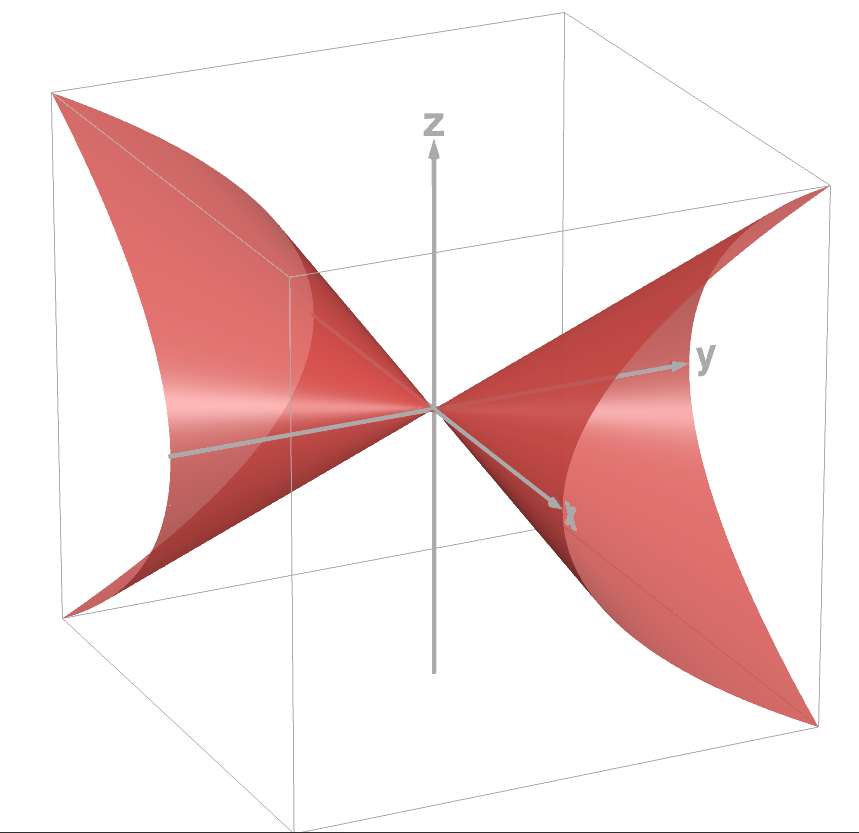
\includegraphics[width=6cm]{Images/quadric cone.png}
    \caption{Quadric cone over the real numbers.}
\end{figure}


$X$ is a toric variety with torus given by the image of\footnote{this map is 2:1, to get the actual parametrization we need
\[\funcDef{\G_m^2}{X}{(s,t)}{(s,st^2,st)}\]
This is related to the fact that $X$ is the quotient $\A^2/\mu_2$ by the action $-1(x,y)=(-x,-y)$.}
\[\funcDef{\G_m^2}{X}{(s,t)}{(s^2,t^2,st)}\]
and action
\[\funcDef{\G_m^2\times X}{X}{((s,t),(x,y,z))}{(sx,st^2y,stz)}\]
\end{example}


\begin{example}
$X=V(xy-zw)\subseteq \A^4$ is a toric variety with torus
\[\funcDef{\G_m^3}{X}{(t_1,t_2,t_3)}{(t_1,t_2,t_3,t_1t_2t_3\ii)}\]
and action 
\[\funcDef{\G_m^3\times X}{X}{((t_1,t_2,t_3),(x,y,z,w))}{(t_1x,t_2y,t_3z,t_1t_2t_3\ii w)}\]
\end{example}


\section{Monoids}

\begin{definition}[Monoid]
A \textbf{monoid} is a set $S$ with an operation $+$, which is commutative, associative and with a neutral element $0\in S$.
\end{definition}

\begin{remark}
The reference book \cite{cox2011toric} calls these \textit{semigroups}.
\end{remark}


\begin{definition}
If $A\subseteq S$ is a subset of a monoid, the \textbf{submonoid generated by $A$ in $S$} is the smallest submonoid which contains $A$. Concretely it is 
\[\ps A=\cpa{\sum_{a\in A} n_a a\mid n_a\in \N,\ n_a=0\text{ for all but finitely many coeff.}}\]
A monoid $S$ is \textbf{finitely generated} if there exists a finite subset $A\subseteq S$ such that $S=\ps A$.
\end{definition}

\begin{remark}
$S$ is a finitely generated monoid if there exists a surjective monoid homomorphism
\[\N^n\onto S.\]
\end{remark}

\begin{definition}
$S$ is an \textbf{affine monoid} if it is finitely generated and it is a submonoid of a lattice $M$.
\end{definition}

\begin{example}
$\N^k\subseteq \Z^k$ is an affine monoid.
\end{example}

\begin{example}
$\znz n$ is a monoid but it is NOT affine because a lattice can't have a submonoid with torsion.
\end{example}

\begin{example}
$\ps{(1,0),(1,1)}\subseteq \N\oplus \znz{2}$ is also not affine because of torsion.
\end{example}

\begin{definition}[Integrality]
A monoid $S$ is \textbf{integral} (or \textbf{cancellative}) if $a+b=a+c\implies b=c$.
\end{definition}

\begin{fact}
A monoid $S$ is affine if and only if $S$ is
\begin{itemize}
\item finitely generated,
\item integral and
\item torsion free.
\end{itemize}
\end{fact}

Let us now define the left adjoint to the forgetful $\Ab\to \Mon$:

\begin{definition}[Associated group]
Let $S$ be a monoid. There is an \textbf{associated abelian group} $S^{gp}$, which is the initial group with a morphism from $S$. Concretely
\[S^{gp}=\frac{\cpa{(s,s')\mid s,s'\in S}}\sim\]
where $(s_1,s'_1)\sim(s_2,s'_2)$ if there exists $s\in S$ such that\footnote{think about localization on rings which are not domains.}
\[s+s_1+s_2'=s+s_2+s_1'.\]
\end{definition}

\begin{remark}
$S^{gp}$ is an abelian group and we have a map $S\to S^{gp}$ given by $s\mapsto [(s,0)]_\sim$.
\end{remark}


\begin{fact}
Any morphism $S\to G$ for $G$ abelian group factors uniquely through $S^{gp}$. More precisely
\[\Hom_{\text{Mon}}(S,G)=\Hom_{\text{Ab}}(S^{gp},G)\]
\end{fact}


\begin{remark}
$S$ is integral if and only if $S\to S^{gp}$ is injective, which happens if and only if $S$ can be injected into an abelian group.
\end{remark}

\subsubsection{Presentations of monoids}
With monoids, the kernel is ``sort of useless"
\begin{example}
Consider
\[\funcDef{\N^2}{\N}{(a,b)}{a+b}\]
this has trivial kernel (preimage of $0$ is just $(0,0)$) but it is far from being injective.
\end{example}

Let $f:S\to S'$ be a surjective homomorphism. What we should look at instead of the kernel for the right analogue of the first isomorphism theorem is
\[E=\cpa{(s,s')\in S\times S\mid f(s)=f(s')}.\]
This set is an equivalence relation on $S\times S$, which is also a submonoid.

\begin{definition}[Congruence relations]
A submonoid of $S\times S$ which defines an equivalence relation is called \textbf{congruence relation}.
\end{definition}

\begin{definition}[Coequalizer]
If $f,g:X\to Y$, the coequalizer is an object $Z$ together with $h:Y\to Z$ such that $h\circ f=h\circ g:X\to Z$ and if $W$ together with $h':Y\to W$ is also such that $h'\circ f=c'\circ g$ then there exists a unique $Z\to W$ making everything commute.
% https://q.uiver.app/#q=WzAsNCxbMCwxLCJYIl0sWzEsMSwiWSJdLFsyLDEsIloiXSxbMiwwLCJXIl0sWzAsMSwiZiIsMCx7Im9mZnNldCI6LTF9XSxbMCwxLCJnIiwyLHsib2Zmc2V0IjoxfV0sWzEsMiwiaCIsMl0sWzEsMywiaCciXSxbMiwzLCJcXGV4aXN0cyEiLDIseyJzdHlsZSI6eyJib2R5Ijp7Im5hbWUiOiJkYXNoZWQifX19XV0=
\[\begin{tikzcd}
	&& W \\
	X & Y & Z
	\arrow["f", shift left, from=2-1, to=2-2]
	\arrow["g"', shift right, from=2-1, to=2-2]
	\arrow["{h'}", from=2-2, to=1-3]
	\arrow["h"', from=2-2, to=2-3]
	\arrow["{\exists!}"', dashed, from=2-3, to=1-3]
\end{tikzcd}\]
\end{definition}

\begin{fact}[]
We can construct quotients of $S$ by a congruence relation $E$ on $S\times S$ by setting it to be the coequalizer of $E\subseteq S\times S\rightrightarrows S$, where the arrows are the two projections from $S\times S$ to $S$.

We call this object the \textbf{quotient of $S$ by $E$} and denote it $S/E$.
\end{fact}

\begin{remark}
If $E$ is the relation constructed from $f:M\onto M'$ homomorphism of abelian groups viewed as monoids then $E=\cpa{(m,m')\in M\times M\mid f(m)=f(m')}=\cpa{(m,m')\mid m-m'\in \ker f}$. It follows that $M'\cong M/\ker f$ is a coequalizer for $E\rightrightarrows M$, so our definition makes sense.
\end{remark}


\begin{definition}[presentation of a monoid]
The monoid associated to
\[\ps{p_1,\cdots, p_r\mid a_1=b_i,\ i\in\cpa{1,\cdots, k}},\]
where $a_i,b_i,\in \ps{p_1,\cdots, p_r}_\N$, is the quotient of $\N^r$ by the congruence relation generated by the $(a_i,b_i)$ in $\N^r\times \N^r$.

A \textbf{presentation} of a monoid $S$ is an isomorphism with a monoid constructed as above.
\end{definition}





\subsection{Monoid algebra}
Since from abelian groups we costructed the group algebra and found connections to geometric objects, we want to generalize that construction to monoids.

\begin{definition}[Monoid algebra]
For a monoid $S$, its \textbf{monoid algebra} $k[S]$ is the $k$-vector space which is freely generated by $\cpa{t^s\mid s\in S}$ and with multiplication induced by the operation on $S$.
\end{definition}


\begin{remark}
In \cite{cox2011toric} they write $\chi^s$ instead of $t^s$ because they think of $S$ inside $M=X(T)$ for some torus.
\end{remark}

\begin{remark}
If $S$ is actually a group then the monoid algebra and group algebras coincide.
\end{remark}


\begin{example}
If $S=\N^n\subseteq \Z^n$ then $k[S]=k[x_1,\cdots, x_n]$.
\end{example}


\begin{proposition}
If $S$ is a monoid with presentation 
\[\ps{p_1,\cdots, p_r\mid a_i=b_i,\ 1\leq i\leq k},\] 
then
\[k[S]=\frac{k[t_1,\cdots, t_r]}{(t^{a_i}-t^{b_i})}\]
where if $a_i=\sum a_{ij}p_j$ we set $t^{a_i}=\prod t_j^{a_{ij}}$.
\end{proposition}
\begin{proof}[Sketch]
Let $R$ be the congruence relation on $\N^r$ generated by $\cpa{(a_i,b_i)}_{1\leq i\leq k}$. Since $R\rightrightarrows \N^r\to S$ is a coequalizer and $S\mapsto k[S]$ is a left adjoint ($\Hom_{\text{Mon}}(S,A)\cong \Hom_{k-\text{Alg}}(k[S],A)$) it follows that
\[k[R]\overset f{\underset g\rightrightarrows} k[\N^r]\to k[S]\] 
is a coequalizer in $k$-algebras, so $k[S]\cong k[\N^r]/I$ where $I=(f(x)-g(x)\mid x\in k[R])$.
\end{proof}



\begin{example}
Let $S=\ps{(2,0),(1,1),(0,2)}\subseteq \Z^2$. This monoid can be seen to be isomorphic to
\[\ps{p,q,r\mid p+q=2r}.\]
It follows that
\[k[S]\cong\frac{k[x,y,z]}{(xy-z^2)},\]
which is the coordinate ring of the quadric cone.
\end{example}

\begin{example}
Consider $S=\ps{2,3}\subseteq \N$, which has presentation
\[\ps{p,q\mid 3p=2q}.\]
It follows that
\[k[S]\cong \frac{k[x,y]}{(x^3-y^2)},\]
the coordinate ring of the cusp curve.
\end{example}


\section{Toric variety associated to a monoid}
Inspired by the success of Cartier duality, we consider the analogous construction with affine monoids. Instead of diagonalizable algebraic groups we will get affine toric varieties:

\begin{proposition}[]\label{PrToricVarietyAssociatedToAffineMonoid}
If $S$ is an affine monoid then
\begin{enumerate}
\item $k[S]$ is a domain and a finitely generated $k$-algebra.
\item $\Spec k[S]$ is an affine toric variety, with torus $\Spec k[S^{gp}]$.
\end{enumerate}
\end{proposition}
\begin{proof}
Let us prove the two propositions
\setlength{\leftmargini}{0cm}
\begin{enumerate}
\item Since $S\subseteq M$, we have an obvious inclusion $k[S]\subseteq k[M]$ and $k[M]$ is a domain, so $k[S]$ also is. Since $S$ is finitely generated, just take the formal variables associated to those generators and they will generate $k[S]$ as a $k$-algebra.
\item The inclusion $S\to M$ must factor through $S\to S^{gp}\to M$ by the universal property. Since $M$ is free of finite rank, $S^{gp}$ also is, thus $T=\Spec k[S^{gp}]=D(S^{gp})$ is a torus (\ref{PrCartierDualOfGeneralFinitelyGeneratedAbelianGroup}) of dimension equal to the rank of $S^{gp}$. Moreover, $k[S^{gp}]$ is a localization of $k[S]$ in a single element: if $\cpa{s_i}_{1\leq i\leq k}$ are generators of $S$ then\footnote{exercise}
\[k[S^{gp}]\cong k[S]_{\prod t^{s_i}}=k[S][t^{-s_1},\cdots,t^{-s_k}]\]
and this isomorphism is induced by the natural map $k[S]\to k[S^{gp}]$. The induced morphism $\Spec k[S^{gp}]\to \Spec k[S]$ is then an open embedding (iso. on local rings).

The translation action of $T$ on itself is the one given by
\[\funcDef{k[S^{gp}]}{k[S^{gp}]\otimes k[S^{gp}]}{t^m}{t^m\otimes t^m},\]
which extends to an action on $\Spec k[S]$ by
\[\funcDef{k[S]}{k[S^{gp}]\otimes k[S]}{t^m}{t^m\otimes t^m},\]
which makes sense because $S\subseteq S^{gp}$.
\end{enumerate}
\setlength{\leftmargini}{0.5cm}
\end{proof}

There is another construction to describe the toric variety associated to the monoid generated by a finite subset $A\subseteq M$ (recall that $M$ is the character lattice of $T$ for some torus).


Consider the morphism 
\[\phi_A:\funcDef{T_N}{(\A^1)^A}{x}{(\chi^a(x))_{a\in A}}\]
\begin{remark}
The image of $\phi_A$ is contained in the standard torus $\imm \phi_A\subseteq (\G_m)^A\subseteq (\A^1)^A$. It follows that $\imm \phi_A$ is also a torus because it is the image of a homomorphism between tori (\ref{PrImageOfTorusInATorusIsATorus}).
\end{remark}

Let $Y_A$ be the closure of $\imm \phi_A$ in $(\A^1)^A$.

\begin{proposition}[]
$Y_A$ is an affine toric variety, with torus given by the one associated to $\Z A\subseteq M$. More precisely, $Y_A\cong \Spec k[\N A]$.
\end{proposition}
\begin{proof}
The morphism $\phi_A$ corresponds to the algebra homomorphism
\[\vp_A:k[x_a\mid a\in A]\to k[M]\]
Note that 
\[\ol{\imm \phi_A}=V(\ker \vp_A)=\Spec \frac{k[x_a\mid a\in A]}{\ker\vp_A}=\Spec \imm \vp_A.\]
It is easy to see that $\imm \vp_A=k[\N A]\subseteq k[M]$. Since $\N A$ is an affine monoid we are done by (\ref{PrToricVarietyAssociatedToAffineMonoid})
\end{proof}

\begin{remark}
The two constructions are the same upon choosing a finite set of generators $A$ for $S$, letting us write $S=\N A$.
\end{remark}

\begin{definition}[Toric ideals]
The ideals of $k[\N^A]$ which give rise to toric varieties are called \textbf{Toric ideals}
\end{definition}

\begin{fact}
Toric ideals are exactly the prime ideals which can be generated by binomials (differences of monic monomials).
\end{fact}

We now want to show that this construction covers all affine toric varieties:

\begin{remark}
The torus $T_N$ acts linearly on its own ring of regular functions $k[M]$ as follows: for $t\in T_N$ and $f\in k[M]$ ($f:T_N\to \A^1$) we define\footnote{the inverse in the definition is not needed since $T_N$ is abelian, but it is put there for consistency with more general theory where it is needed to verify that the map given is indeed a left-action.}
\[t\cdot f:\funcDef{T_N}{\A^1}{p}{f({t\ii\cdot p})}\]
where the product $t\ii\cdot p$ is the product of $T_N$ as an algebraic group.
\end{remark}

\begin{lemma}[]\label{LmSimultaneousEigenvectorsForActionOfTorusAreTheCharacters}
The only simultaneous eigenvectors of the action $T_N\acts k[M]$ given above are the characters.
\end{lemma}
\begin{proof}
Note that $t\cdot \chi^m (p)=\chi^m(t\ii\cdot p)=\chi^m(t\ii)\chi^m(p)$ on the torus, thus $t\cdot \chi^m=\chi^m(t\ii) \chi^m$, that is, characters are simultaneous eigenvectors for this action of $T_N$. 

Let us now prove that they are the only ones (up to scalars):
if $\sum a_m \chi^m$ in $k[M]$ is a simultaneous eigenvector then 
\[\al(t)\pa{\sum a_m \chi^m}=t\cdot \pa{\sum a_m \chi^m}=\sum \chi^m(t\ii)a_m \chi^m\]
for some function $\al:T_N\to k$, thus $a_m\al(t)=a_m\chi^m(t\ii)$ for all $m$. If $a_{m_1}\neq 0\neq a_{m_2}$ then $\chi^{m_1}(t\ii)=\al(t)=\chi^{m_2}(t\ii)$, so $m_1=m_2$ and thus the simultaneous eigenvector we chose must be of the form $a_m \chi^m$ for some $m\in M$.
\end{proof}

\begin{lemma}
If $A\subseteq k[M]$ is a subspace which is stable under the action above then
\[A=\bigoplus_{t^m\in A}k t^m,\]
that is, $A$ is generated by characters.
\end{lemma}
\begin{proof}
Call $A'=\bigoplus_{t^m\in A}k t^m$. Clearly $A'\subseteq A$ so we just need the other inclusion. Pick $f\in A$ and write
\[f=\sum_{m\in B}c_m t^m\]
for $B\subseteq M$ finite and such that $c_m\neq 0$ for all $m\in B$. Note that
\[f\in A\cap \ps{t^m\mid m\in B}:=V.\]
This intersection is a finite dimensional $k$-vector space which is stable under the $T_N$-action, so it is a finite dimensional representation of $T_N$. By proposition (\ref{PrRepresentationsOfToriSplit}) it follows that $V$ is generated by simultaneous eigenvectors of the action, which are the $t^m$ by the lemma above. Writing what we have just said in symbols: 
\[f\in V=\bigoplus_{\smat{m\in B\ s.t.\\ t^m\in A}}kt^m\subseteq \bigoplus_{t^m\in A}k t^m=A'.\]
\end{proof}

\begin{theorem}[]\label{ThAffineToricVarietiesComeFromAffineMonoids}
All affine $T_N$-toric varieties are isomorphic to one of the form $\Spec k[S]$ for some monoid $S\subseteq M=X(T_N)$.
\end{theorem}
\begin{proof}
If $X=\Spec A$ is an affine toric variety, then $A\subseteq k[M]$ is stable for the action of $T_N$ on $k[M]$. This is because $\cdot t\ii:T_N\to T_N$ extends to $X$ by definition of toric variety.
By the lemma above
\[A=\bigoplus_{t^m\in A}k t^m=k[S],\]
where $S=\cpa{m\in M\mid t^m\in A}$, which is a submonoid of $M$ because $A$ is an algebra.

Since $A$ is finitely generated, there exist $f_1,\cdots, f_k$ such that $A=k[f_1,\cdots, f_k]$. By replacing each $f_i$ with all the characters that you need to write it out, we can assume that the $f_i$ are all of the form $t^m$.

It is now easy to check that the corresponding exponents generate $S$.
\end{proof}























\chapter{Projective toric varieties}

\section{Introduction}
\begin{definition}[]
A \textbf{projective toric variety} is an irreducible, normal projective variety $X$ equipped with an open embedding $T\subseteq X$ of an algebraic torus such that the translation action of $T$ extends to $X$.
\end{definition}

\begin{remark}
Projective space $\Pj^n$ is a projective toric variety with torus given by
\[\Pj^n\bs V(x_0\cdots x_n).\]
This is the same torus that we get on all the affine charts.

The translation action extends as follows:
\[\funcDef{\G_m^n\times \Pj^n}{\Pj^n}{((a_1,\cdots, a_n),[x_0,\cdots, x_n])}{[x_0,a_1x_1,\cdots, a_n x_n]}\]
The character lattice of this torus $T_{\Pj^n}$ can be thought of as follows: recall that we have
\[\A^{n+1}\nz\xrightarrow{\pi}\frac{\A^{n+1}\nz}{\G_m}\cong \Pj^n\]
and this induces
\[0\to \G_m\to \G_m^{n+1}\to T_{\Pj^n}\to0\]
where the first inclusion is via matricies of the form $\la I$. Dually we get a short exact sequence of the character lattices
\[0\to M_{\Pj^n}\to \Z^{n+1}\to \Z\to 0\]
so we may write
\[M_{\Pj^n}=\cpa{(a_0,\cdots, a_n)\in \Z^{n+1}\mid \sum a_i=0}\subseteq \Z^{n+1}.\]
\end{remark}

Now, given a finte subset $A\subseteq M$ (let us write $A=\cpa{a_1,\cdots, a_s}$) we can consider
\[\vp_A:\funcDef{T_N}{\G_m^s}{t}{(\chi^{a_1}(t),\cdots, \chi^{a_s}(t))}\]
and then the composition
\[\psi_A:T_N\xrightarrow{\vp_A}\G_m^s\inj \A^2\nz\onto \Pj^{s-1}.\]
The closure of the image of $\psi_A$ inside $\Pj^{s-1}$ is the \textbf{projective toric variety $X_A$ associated to $A$}

\begin{proposition}[]\label{PrProjectiveToricVarietyAssociatedToFiniteSubsetOfCharacters}
$X_A$ as above is a projective toric vriety. $\dim X_A=\dim \mathrm{Affspan}_\R{A}$ where the last notation means \textit{the affine subspace generated by $A$} in $M_\R$.
\end{proposition}
\begin{proof}
Let $T$ be the image of $T_N\to \G_m^s\to T_{\Pj^{s-1}}$, which is still a torus by (\ref{PrImageOfTorusInATorusIsATorus}). Note that $X_A$ is the closure of $T$ in $\Pj^{s-1}$.

If $t\in T$, $t\cdot T=T\subseteq X_A$ and $\ol{t\cdot T}=t\cdot \ol T=t\cdot X_A$, so $t\cdot X_A\subseteq X_A$, but the same holds for $t\ii$, thus the action extends.

$\dim X_A=\dim T=\rnk_\Z M'$ where $M'=X(T)$. We can compute $M'$:
% https://q.uiver.app/#q=WzAsMyxbMCwwLCJUX04iXSxbMSwwLCJUIl0sWzEsMSwiVF97XFxQal57cy0xfX0iXSxbMCwyXSxbMSwyLCIiLDMseyJzdHlsZSI6eyJ0YWlsIjp7Im5hbWUiOiJob29rIiwic2lkZSI6InRvcCJ9fX1dLFswLDEsIiIsMyx7InN0eWxlIjp7ImhlYWQiOnsibmFtZSI6ImVwaSJ9fX1dXQ==
\[\begin{tikzcd}
	{T_N} & T \\
	& {T_{\Pj^{s-1}}}
	\arrow[two heads, from=1-1, to=1-2]
	\arrow[from=1-1, to=2-2]
	\arrow[hook, from=1-2, to=2-2]
\end{tikzcd}\]
yields dually (apply $X(\cdot)$ functor)
% https://q.uiver.app/#q=WzAsMyxbMSwxLCJNX3tcXFBqXntzLTF9fSJdLFsxLDAsIk0nIl0sWzAsMCwiTSJdLFswLDJdLFsxLDIsIiIsMyx7InN0eWxlIjp7InRhaWwiOnsibmFtZSI6Imhvb2siLCJzaWRlIjoiYm90dG9tIn19fV0sWzAsMSwiIiwzLHsic3R5bGUiOnsiaGVhZCI6eyJuYW1lIjoiZXBpIn19fV1d
\[\begin{tikzcd}
	M & {M'} \\
	& {M_{\Pj^{s-1}}}
	\arrow[hook', from=1-2, to=1-1]
	\arrow[from=2-2, to=1-1]
	\arrow[two heads, from=2-2, to=1-2]
\end{tikzcd}\]
so $M'$ is the image of $M_{\Pj^{s-1}}\to M$, which is induced by the map $\Z^s\to M$ which sends $e_i$ to $a_i$, so the image is exactly
\[\cpa{\sum k_i a_i\mid \sum k_i=0}=\ps{a_i-a_j\mid i\neq j}\subseteq M.\]
Upon tensoring this with $\R$ we get the vector subspace of $M_\R$ associated to the affine subspace generated by $A$.
\end{proof}


\begin{remark}
One may expect $Y_A\subseteq \A^{s}$ to be related to the affine cone over $X_A$. The two are the same if and only if $I(Y_A)$ is homogeneous iff exists $n\in N$ and $k$ positive such that **************
(i.e. $A$ is contained in an affine hyperplane of $M_\R$).
\end{remark}

\begin{remark}
The toric variety $X_A\subseteq \Pj^{s-1}$ is covered by affine toric varieties, given by the intersections $X_A\cap U_i$. The $X_A\cap U_i$ are indeed affine and they are toric because they all contain $T$. In fact $X_A\cap U_i=\ol{T}^{U_i}$.
\end{remark}


\begin{proposition}[]\label{PrMonoidOfAffineChartOfProjectiveToricVariety}
The monoid of $X_A\cap U_i$ is the submonoid $A_i$ of $M$ generated by $a_j-a_i$ for $j\neq i$.
\end{proposition}
\begin{proof}
It suffices to show that $X_A\cap U_i$ is the closure of the image of $T_N\to U_i\to \A^{s-1}$. If $t\in T_N$ then the maps go
\[t\mapsto [\chi^{a_1}(t),\cdots,\chi^{a_s}(t)]\mapsto (\chi^{a_1-a_i}(t),\cdots, \chi^{a_s-a_i}(t))\]
and this is exactly what we want.
\end{proof}


\begin{remark}
$A_i^{gp}$ is exactly the character lattice of $T$ that we found the proof before.
\end{remark}



\begin{example}[Rational normal curve]
Let $A\subseteq \Z^2$ be the subset given by $A=\cpa{(0,d),(1,d-1),\cdots, (d,0)}$. The affine toric variety $Y_A$ is what we called \textit{rational normal cone of degree $d$}.

The projective toric variety $X_A$ is called the \textbf{rational normal curve of degree $d$} in $\Pj^d$ and $Y_A$ is its affine cone in $\A^{d+1}$.
\end{example}

\begin{example}
Let $A=\cpa{e_1,e_2,e_3,e_1+e_2-e_3}$. The affine toric variety is
\[Y_A=\Spec\frac{k[x,y,z,w]}{(xy-zw)}\subseteq\A^4\]
The projective toric variety $X_A$ is the one in $\Pj^3$ given by the same equation $xy=zw$. This is actually isomorphic to $\Pj^1\times \Pj^1$ via the Segre embedding
\[\funcDef{\Pj^1\times \Pj^1}{\Pj^3}{([y_0,y_1],[z_0,z_1])}{[y_0z_0,y_1z_1,y_0z_1,y_1z_0]}\]
\end{example}


\section{Polytopes}
We have seen that affine toric varieties are described by cones. For projective toric varieties we have a similar correspondence with polytopes.

\begin{definition}[]
A \textbf{polytope} in $M_\R$ is the convex hull of a finite subset $A\subseteq M_\R$, i.e.
\[P=\Conv(A)=\cpa{\sum_{m\in M}\la_m m\mid \la_m\geq 0,\ \sum \la_m=1}.\]
\end{definition}

Given such a $P$ we can construct a cone
\[\Cone(A\times \cpa{1})\subseteq M_\R\oplus \R.\]
We can recover the polytope by slicing the cone at height 1.

This corresponcence is sometimes useful to prove things about polytopes by reducing to the case of cones.

\begin{definition}[]
The \textbf{dimension} of a polytope $P$ is the dimension of the smalled affine subspace of $M_\R$ which contains $P$.
\end{definition}

\begin{definition}[]
Let $u\in N_\R$ and $b\in \R$. They determine an \textbf{affine hyperplane}
\[H_{u,b}=\cpa{m\in M_\R\mid \ps{m,u}=b}\subseteq M_\R\]
and a \textbf{closed half-space}
\[H_{u,b}^+=\cpa{m\in M_\R\mid \ps{m,u}\geq b}\subseteq M_\R\]
\end{definition}

\begin{definition}[]
A subset $Q\subseteq P$ is a \textbf{face} if there exist $n\in N_\R$ and $b\in \R$ such that $P\subseteq H_{u,b}^+$ (in this case we say that $H_{u,b}$ is a \textbf{supporting hyperplane}) and $Q=P\cap H_{u,b}$.
\end{definition}

\begin{remark}
Faces of a polytope are polytopes. Moreover, if $P=\Conv(A)$ then $Q=\Conv(A\cap H_{u,b})$ for $H_{u,b}$ supporting hyperplane which defines $Q$.
\end{remark}

\begin{definition}[]
Faces of dimension $0$ are called \textbf{vertices}, those of dimension 1 are \textbf{edges} and those of codimension 1 are \textbf{facets}.
\end{definition}

\begin{fact}
If $P$ is a polytope then
\begin{itemize}
\item $P=\Conv(\text{vertices of }P)$
\item If $P=\Conv(A)$ and $v\in P$ is a vertex then $v\in A$
\item if $Q\leq P$ then 
\[\cpa{\text{faces of }Q}=\cpa{\text{faces of $P$ contained in $Q$}}\]
\item if $Q<P$ (proper face) then 
\[Q=\bigcap_{\smat{F\text{ facet of $P$}\\ Q\leq F}}F\]
\item a polytope is a finite intersection of closed half-spaces
\item any finite intersection of closed half-spaces which is bounded is a polytope
\end{itemize}
\end{fact}

\begin{fact}
When $P$ is full-dimensional, each facet $F$ has a \textit{unique} supporting hyperplane.
\end{fact}

\begin{notation}
If $F$ is a facet of $P$ full-dimensional we use $H_F^+$ to denote the associated supporting hyperplane and we denote by $u_F\in N_\R$, $a_F\in \R$ the pair such that
\[H_F^+=H_{u_F,-a_F}.\]
The sign of $a_F$ is that way just for convention, it will make some computations easier later on. Note that the pair $(u_F,a_F)$ is not unique but it become unique up to positive scaling.
\end{notation}

\begin{definition}[]
A polytope $P$ is a \textbf{lattice polytope} if there exists $A\subseteq M$ finite such that $P=\Conv(A)$.
\end{definition}

\begin{remark}
This is equivalent to saying that all vertices of $P$ lie in $M$.
\end{remark}

\begin{fact}
The following propositions hold
\begin{itemize}
\item Faces of lattice polytopes are lattice polytopes
\item in the description of $P$ as $P=\bigcup_{i=1}^sH_{u_i,s_i}^+$ we can assume that the $u_i$ are also points in the lattice $N$
\item If $P$ is a full-dimensional lattice polytope we have a presentation 
\[P=\bigcup_{F\text{ facet of $P$}}H_F^+\]
and we can assume that $u_F$ is the minimal ray generator of $\Cone(u_F)$.
\item The presentation above for a given $P$ is unique and the pairs $(u_F,a_F)$ chosen as above ($u_F$ minimal ray generator) are unique. 
\[P=\cpa{m\in M_\R\mid \ps{m,u_F}\geq -a_F\ \forall F\text{ facet of }P}.\]
\end{itemize}
\end{fact}

\begin{example}
The standard $n$-dimensional simplex $\Delta_n=\Conv(0,e_1,\cdots, e_n)$ is a polytope of dimension $n$. It has exactly $n+1$ vertices.
\end{example}


\section{Toric varieties from polytopes}
Now the idea is, given a lattice polytope $P$, which we assume to be full-dimensional, is to take $X_{P\cap M}$

\begin{remark}
If $M$ is a lattice and $P$ is a lattice polytope in $M_\R$, $P\cap M$ is a finite set.
\end{remark}

This works, but if we want the combinatorics of $P$ to reflect the geometry of $X_{P\cap M}$ correctly, we need $P$ to have ``enough" lattice points.

There are two notions that are related to this issue: \textit{normality} and \textit{very ampleness}. We will only discuss the second one.

\subsection{Very ampleness}

\begin{definition}[]
A lattice polytope is \textbf{very ample} if for all vertices $v$ of $P$, the monoid
\[\ps{P\cap M-v}=\ps{m-v\mid m\in P\cap M}\]
is saturated.
\end{definition}

\begin{remark}
The idea of taking the difference with $v$ translates to making $v$ the origin

PICTURE IN THE NOTES
\end{remark}

\begin{definition}[]
If $P,Q$ are subsets of $M_\R$, their \textbf{Minkowski sum} is
\[P+Q=\cpa{p+q\mid p\in P,\ q\in Q}\]
\end{definition}
\begin{remark}
If $P=\Conv(A)$ and $Q=\Conv(B)$ then $P+Q=\Conv(A+B)$.
\end{remark}

\begin{notation}
If $k>0$ and $P=\Conv(A)$, then we set $kP$ to be the polytope defined by $\Cone(\cpa{ka\mid a\in A})$.
If $k\in \N$, this also coincides with the iterated Minkowski sum
\[\under{k\text{ times}}{P+\cdots+P}=\cpa{m_1+m_2+\cdots+m_k\mid m_i\in P}.\]
\end{notation}

\begin{remark}
If $P$ is defined by $\cpa{\ps{m,n_i}\geq b_i\mid i\in\cpa{1,\cdots, s}}$ then
\[kP=\cpa{\ps{m,n_i}\geq kb_i\ \forall i}\]
\end{remark}

\begin{fact}
Let $P\subseteq M_\R$ be a full-dimensional lattice polytope with $\rnk M\geq 2$. Then $kP$ is very ample for all $k\geq n-1$.
\end{fact}
\begin{remark}
If $\rnk M=1$ we have no issue in finding a very ample multiple.
\end{remark}

\subsection{The projective variety}
Let $P$ be a full-dimensional lattice polytope. The associated projective variety is
\[X_P=X_{(kP)\cap M}\]
for $k\in\N$ such that $kP$ is very ample.

\begin{remark}
This will yield a well defined abstract variety, though the embedding in the ambient projective spaces change with respect to $k$.
\end{remark}


Recall that $X_A\subseteq \Pj^{s-1}$ is covered by affine toric varieties: via (\ref{PrMonoidOfAffineChartOfProjectiveToricVariety}) we have (for $A=\cpa{a_1,\cdots, a_s}$)
\[X_A=\bigcup_{i=1}^s X_A\cap U_i\]
\begin{lemma}\label{LmWeOnlyNeedAffineChartsOfVertices}
If $A=P\cap M$ then
\[X_A=\bigcup_{a_i\text{ vertex of $P$}}X_A\cap U_i\]
\end{lemma}
\begin{proof}
Let $\cpa{a_j}_{j\in J}$ be the vertices of $P$. Fix $a_i\in A\bs \cpa{a_j}_{j\in J}$. We want to find $j\in J$ such that $X_A\cap U_i\subseteq X_A\cap U_j$.
Note that (exercise)
\[P\cap M_\Q=\cpa{\sum_{j\in J}r_j a_j\mid r_j\in \Q_{\geq 0},\ \sim r_j=1},\]
so we can write
\[a_i=\sum_{j\in J}r_j a_j.\]
If we clear the denominators we get
\[ka_i=\sum k_j a_j,\quad k, k_j\in \N,\ k\neq 0,\ \sum k_j=k.\]
From this we get
\[\sum_{j\in J}k_j(a_j-a_i)=0.\]
Let $j_0\in J$ be such that $k_{j_0}\neq 0$. It follows that
\[k_{j_0}(a_i-a_{j_0})=\sum_{j\in J\bs\cpa{j_0}}k_j(a_j-a_i)\]
so $a_i-a_{j_0}\in S_i=\ps{a_k-a_i\mid k\neq i}$ and $S_i$ is the monoid which corresponds to $X_A\cap U_i$. Note that $a_{j_0}-a_i\in S_i$ by definition, so also having $k_{j_0}(a_i-a_{j_0})\in S_i$ means that $a_{j_0}-a_i$ is invertible in $S_i$.

Note that $k[S_i]_{t^{a_{j}-a_i}}$ is the coordinate ring of $X_A\cap U_i\cap U_j$, but for $j_0$
\[k[S_i]_{t^{a_{j_0}-a_i}}=k[S_i]\]
so $X_A\cap U_i\cap U_{j_0}=X_A\cap U_i$, that is, $X_A\cap U_i\subseteq X_A\cap X_{j_0}$.
\end{proof}


\begin{theorem}[]\label{ThAffineChartsOfProjectiveToricVarietyFromVeryAmplePolytope}
Assume $P$ is a very ample full-dimensional lattice polytope. Then
\begin{itemize}
\item if $a_i\in P\cap M$ is a vertex, then $X_{P\cap M}\cap U_i\cong U_{\sigma_i}=\Spec k[\sigma_i^\vee\cap M]$ where $\sigma_i\subseteq N_\R$ is the strongly convex cone which is dual to $C_i=\Cone(P\cap M-a_i)$. Moreover $\dim\sigma_i=n$
\item The torus of $X_{P\cap M}$ is $T_N$.
\end{itemize}
\end{theorem}
\begin{proof}
Since $a_i$ is a vertex and $P$ is full-dimensional, $C_i$ is strongly convex and full-dimensional. Now $S_i$ (monoid that corresponds to $X_A\cap U_i$) is a submonoid $S_i\subseteq C_i\cap M=\sigma_i^\vee\cap M$ by construction.

Since $P$ is very ample, $S_i$ is saturated and as in a proof which we have seen ($2\implies 3$ from (\ref{PrCriteriaForNormalAffineToricVariety})) it follows that we have equality.

The fact that the torus is $T_N$ follows from the fact that the $\sigma_i$ are strictly convex and that the torus of $X_A$ is the same as the torus of $X_A\cap U_i$ for any $i$.
\end{proof}


The cones $\sigma_i$ assemble into the \textbf{normal fan} of the polytope $P$:
if we write \[P=\cpa{m\in M_\R\mid \ps{m,u_F}\geq -a_F\ \forall \text{$F$ facet}}\]
and fix a vertex $v\in P$, at $v$ we have a cone
\[C_v=\Cone(P\cap M-v)\]
and $\sigma_v=C_v^\vee$ as in the proof.
There is a bijection
\[\correspDef{\cpa{Q\leq P,\ v\in Q}}{\cpa{\tau\leq C_v}}{Q}{Q_v=\Cone(Q\cap M-v)}{Q_\tau=(\tau+v)\cap P}{\tau}\]
This bijection preserves inclusions, intersection, dimension etc.

PICTURE

In particular facets of $C_v$ correspond to facets of $P$ containing $v$, so
\[C_v=\cpa{m\in M_\R\mid \ps{m,u_F}\geq 0\ \forall \text{facet containing $v$}}.\]
So $\sigma_v=C_v^\vee=\Cone(u_F\mid v\in F)$.

We can extend this association $vertices\to cones$ to all faces of $P$ as follows:
\[Q\leq P\mapsto \sigma_Q=\Cone(u_F\mid Q\subseteq F)\]

\begin{example}
If $F\leq P$ is a facet, $\sigma_F$ is the ray generated by $u_F$. If $Q=P$ then $\sigma_P=\Cone(\emptyset)=\cpa{0}$.
\end{example}


\begin{definition}[]
The cones $\cpa{\sigma_Q\mid Q\leq P}$ give the \textbf{normal fan} of $P$, denoted $\Sigma_P$.
\end{definition}

\begin{definition}[]
A \textbf{fan} $\Sigma$ in $N_\R$ is a finite collection of strongly convex cones such that
\begin{enumerate}
\item for all $\sigma,\sigma'\in \Sigma$, $\sigma\cap \sigma'$ is a face of both
\item if $\sigma\in \Sigma$ and $\tau\leq \sigma$ then $\tau \in \Sigma$.
\end{enumerate}
\end{definition}


\begin{example}
PICTURE
\end{example}


\begin{proposition}[]\label{PrDualityOfFacesOfACone}
If $\tau\leq \sigma$ there is a dual face $\tau^\ast\leq \sigma^\vee$ defined as $\sigma^\vee\cap ((\Span_\R\tau)^\perp)$. This construction gives an inclusion-reversing bijection between faces of $\sigma$ and faces of $\sigma^\vee$.
\end{proposition}
\begin{example}
DRAWING FROM LECTURES
\end{example}


\begin{remark}
For all $u\in N_\R\nz$ there exists a unique $b\in \R$ such that $H_{u,b}^+\supseteq P$ and $H_{u,b}\cap P\neq \emptyset$.
\end{remark}

\begin{theorem}[]\label{ThNormalFanOfPolytopeIsAFan}
The normal fan of a polytope $P$ is a fan.
\end{theorem}
\begin{proof}[Sketch]
We have the following steps:
\setlength{\leftmargini}{0cm}
\begin{enumerate}
\item Note that
\[\sigma_Q=\cpa{u\in N_\R\mid \exists b\in \R\ s.t.\ H_{u,b}\text{ is supporting and }Q\subseteq H_{u,b}\cap P},\]
indeed
\setlength{\leftmargini}{0cm}
\begin{itemize}
\item[$\boxed{\subseteq}$] take $u\in \sigma_Q$, then $u=\sum_{Q\subseteq F}\la_F u_F$ for $\la_F\geq 0$. Let $b_0=\sum_{F\text{ facet}, Q\subseteq F}-\la_F a_F\in \R$. By construction\footnote{$\ps{m,u}=\sum \la_F\ps{m,u_F}\geq -\sum \la_F a_F=b_0$}, $P\subseteq H_{u,b_0}^+$ and $Q\subseteq H_{u,b_0}\cap P$ because $Q=\bigcap_{Q\subseteq F} F$
\item[$\boxed{\supseteq}$] Assume that $b\in \R$ is such that $H_{u,b}$ is supporting and $Q\subseteq H_{u,b}\cap P$. Let $v$ be a vertex of $Q$ (which is also a vertex of $P$). From $P\subseteq H_{u,b}^+$ and $P\in H_{u,b}$ it follows that $C_v\subseteq H_{u,0}^+$, i.e. $u\in (C_v)^\vee=\sigma_v=\Cone(u_F\mid v\in F)$, thus $u=\sum_{v\in F} \la_F u_F$ with some $\la_F\geq 0$. We have to show that if $Q\not\subseteq F$ then $\la_F=0$: fix $F_0$ such that $Q\not\subseteq F_0$ and $p\in Q\bs F_0$. $p,v\in Q\subseteq H_{u,b}$, so
\[b=\ps{p,u}=\sum \la_F\ps{p,u_F}\]
but also
\[b=\ps{v,u}=\sum \la_F\ps{v,u_F}=-\sum_{v\in F}\la_F a_F\]
so $\sum_{v\in F}\la_F\ps{p,u_F}=-\sum_{v\in F}\la_F a_F$, but $\ps{p,u_F}\geq -a_F$ for all $F$, so we get equality everywhere $\la_F\neq 0$. Since $p\notin F_0$ we have $\ps{p,u_{F_0}}>-a_{F_0}$, so $\la_{F_0}=0$.
\end{itemize}
\setlength{\leftmargini}{0.5cm}
\item If $Q\leq P$ and $F\leq P$ facet then $u_F\in \sigma_Q$ if and only if $Q\subseteq F$
\item if $Q\subseteq Q'$ then $\sigma_{Q'}\leq \sigma_{Q}$ and all faces of $\sigma_Q$ are of this form\footnote{for this you need duality of faces for a cone $\sigma$ (\ref{PrDualityOfFacesOfACone}).}.
\item $\sigma_Q\cap \sigma_{Q'}=\sigma_{Q''}$ where $Q''$ is the smallest face of $P$ which contains both $Q$ and $Q'$.
\end{enumerate}
\setlength{\leftmargini}{0.5cm}
\end{proof}


\begin{remark}
$\sigma_Q$ is strictly convex because each $\sigma_Q$ is a face of some $\sigma_v$ and $\sigma_v$ is strictly convex because $P$ is full-dimensional.
\end{remark}

\begin{remark}
The $\sigma_v$ are the \textbf{maximal cones} of $\Sigma_P$ since any other $\sigma_Q$ is a face of some $\sigma_v$.
\end{remark}


\begin{definition}[]
A fan $\Sigma$ in $N_\R$ is called \textbf{complete} if
\[\abs{\Sigma}=\bigcup_{\sigma\in \Sigma}=N_R\]
\end{definition}



\begin{proposition}[]
If $P$ is a full-dimensional lattice polytope then $\Sigma_P$ is complete.
\end{proposition}
\begin{proof}
Fix $u\in N_\R\nz$ and set $b=\min\cpa{\ps{v,u}\mid v\text{ vertex of $P$}}$. Then $P\subseteq H_{u,b}^+$ and there exists $v_0$ vertex such that $\ps{v_0,u}=b$, that is, $v_0\in H_{u,b_0}$. From what we have seen, this implies that $u\in\sigma_{v_0}\subseteq \abs{\Sigma_P}$.
\end{proof}

\begin{remark}
The normal fan of $P$ is invariant with respect to dilations and translations by integral vectors, that is, 
\[\Sigma_P=\sigma_{kP+m}\]
for any $k\in \N$ and $m\in M$.
\end{remark}

Together with the next proposition, this implies that the projective toric varieties $X_{kP}, X_P,\ X_{P+m}$ are all abstractly isomorphic. The only difference is the embedding in projective space.


\begin{proposition}[]\label{PrIntersectionOfAffineChartsForProjectiveToric}
If $P$ is a very ample full-dimensional lattice polytope. Let $v\neq w$ be vertices of $P$ and let $Q$ be the smallest face of $P$ which contains both. Then\footnote{$\sigma_Q=\sigma_v\cap \sigma_w$ so intersections at the level of cones in the fan describe how the affine patches of the toric variety are glued together.}
\[X_{P\cap M}\cap U_v\cap U_w\cong U_{\sigma_Q}=\Spec k[\sigma_Q^\vee\cap M].\]
\end{proposition}
\begin{proof}
We have inclusions
% https://q.uiver.app/#q=WzAsNSxbMSwyLCJYX3tQXFxjYXAgTX1cXGNhcCBVX3ZcXGNhcCBVX3ciXSxbMCwxLCJYX3tQXFxjYXAgTX1cXGNhcCBVX3YiXSxbMCwwLCJVX3tcXHNpZ21hX3Z9Il0sWzIsMSwiWF97UFxcY2FwIE19XFxjYXAgVV93Il0sWzIsMCwiVV97XFxzaWdtYV93fSJdLFsyLDEsIj0iLDMseyJzdHlsZSI6eyJib2R5Ijp7Im5hbWUiOiJub25lIn0sImhlYWQiOnsibmFtZSI6Im5vbmUifX19XSxbMSwwLCJcXHN1cHNldGVxIiwzLHsic3R5bGUiOnsiYm9keSI6eyJuYW1lIjoibm9uZSJ9LCJoZWFkIjp7Im5hbWUiOiJub25lIn19fV0sWzQsMywiPSIsMyx7InN0eWxlIjp7ImJvZHkiOnsibmFtZSI6Im5vbmUifSwiaGVhZCI6eyJuYW1lIjoibm9uZSJ9fX1dLFswLDMsIlxcc3Vic2V0ZXEiLDMseyJzdHlsZSI6eyJib2R5Ijp7Im5hbWUiOiJub25lIn0sImhlYWQiOnsibmFtZSI6Im5vbmUifX19XV0=
\[\begin{tikzcd}
	{U_{\sigma_v}} && {U_{\sigma_w}} \\
	{X_{P\cap M}\cap U_v} && {X_{P\cap M}\cap U_w} \\
	& {X_{P\cap M}\cap U_v\cap U_w}
	\arrow["{=}"{marking, allow upside down}, draw=none, from=1-1, to=2-1]
	\arrow["{=}"{marking, allow upside down}, draw=none, from=1-3, to=2-3]
	\arrow["\supseteq"{marking, allow upside down}, draw=none, from=2-1, to=3-2]
	\arrow["\subseteq"{marking, allow upside down}, draw=none, from=3-2, to=2-3]
\end{tikzcd}\]
and we identify the double intersection both with $(U_{\sigma_v})_{t^{w-v}}\subseteq U_{\sigma_v}$ and $(U_{\sigma_w})_{t^{v-w}}\subseteq U_{\sigma_w}$. 

We need to show that, for instance, $(U_{\sigma_v})_{t^{w-v}}$ can be identified with $U_{\sigma_{Q}}$. Note that $w-v\in C_v=\sigma_v^\vee$ so $\tau:=H_{w-v}\cap \sigma_v\leq \sigma_v$. We saw that $(U_{\sigma_v})_{t^{w-v}}\cong U_\tau$ (\ref{ThAffineChartsOfProjectiveToricVarietyFromVeryAmplePolytope}).


Let us check that $\tau=\sigma_Q$. We know that $\sigma_Q=\sigma_v\cap \sigma_w$ from the proof that the normal fan is a fan (\ref{ThNormalFanOfPolytopeIsAFan}), i.e. we want $H_{w-v}\cap \sigma_v=\sigma_w\cap \sigma_v$.
\setlength{\leftmargini}{0cm}
\begin{itemize}
\item[$\boxed{\subseteq}$] If $n\in H_{w-v}\cap \sigma_v\nz$ then there exists a unique $b\in\R$ such that $H_{u,b}$ is supporting for $P$ and $u\in \sigma_v$ implies $v\in H_{u,b}$ (proposition from little ago). Also $u\in H_{w-v}$, that is, $\sp{w,u}=\ps{v,u}$, so putting the two facts together $\ps{w,u}=b$, that is, $u\in \sigma_w$.
\item[$\boxed{\supseteq}$] If $u\in \sigma_v\cap \sigma_w\nz$ and $b\in \R$ such that $H_{u,b}$ supporting then $u\in \sigma_v$ implies $v\in H_{u,b}$ and so .................... $\ps{w-v,u}=0$ which implies $u\in H_{w-v}$.
\end{itemize}
\setlength{\leftmargini}{0.5cm}
\end{proof}

\begin{remark}
What we are sayng is that the toric variety depends only on the fan in some sense, not the polytope.
\end{remark}



\begin{remark}
This shows that for a full-dimensional lattice polytope $P$, $X_P=X_{(kP)\cap M}$ where $kP$ is very ample as an abstract variety / scheme only depends on the normal fan $\Sigma_P$ and can be constructed directly from it.
\end{remark}


\begin{example}
Let $P=\Delta_n=\Cone(0,e_1,\cdots, e_n)\subseteq \R^n$. Let $A=\Delta_n\cap \Z^n=\cpa{0,e_1,\cdots, e_n}$.
\[\phi_A:\funcDef{\G_m^n}{\Pj^n}{(a_1,\cdots, a_n)}{[1,a_1,a_2,\cdots, a_n]}\]
and this is exactly an embedding of the torus of $\Pj^n$, which is dense, so $X_{\Delta_n}=\Pj^n$.


Let us now try $k\Delta_n$. Then $X_{k\Delta_n}$ is still isomorphic to $\Pj^n$ but it is embedded in $\Pj^{\binom{n+k}k-1}$ via the Veronese embedding. For example, for $n=k=2$ we have $2\Delta_2\cap \Z^2=\cpa{(0,0),(1,0),(2,0),(0,1),(0,2),(1,1)}$ and
\[\phi_A:\funcDef{\G_m^2}{\Pj^5}{(a,b)}{[1,a,a^2,b,b^2,ab]}\]
This extends to
\[\funcDef{\Pj^2}{\Pj^5}{[x_0,x_1,x_2]}{[x_0^2,x_0x_1,x_1^2,x_0x_2,x_2^2,x_1x_2]}\]
which is the Veronese embedding.
\end{example}


\begin{example}
Consider the trapezoids given by the convex hull of 
\[(0,1), (0,0), (0,b), (0,a)\]
and let $X_{a,b}$ be the associated toric variety. If $b-a=b'-a'$ then $X_{a,b}\cong x_{a',b'}$ because the fan doesn't change (even though we it's not necessarily the case that we get between such isomorphic polytope by scaling and translating).

This toric variety is called Hirzebruch surface $H_r$ where $r=b-a\in \N$. Another description for it is $\Pj(\Oc\oplus \Oc(-r))$.
\end{example}





\begin{proposition}[]\label{PrSmoothnessAndNormalityOfProjectiveToricVarieties}
If $P$ is a full-dimensional lattice polytope, then $X_P$ is normal (because the affine pieces are of the form $U_{\sigma_v}$ for $\sigma_v$ stictly convex) and $X_P$ is smooth if and only if $\Sigma_P$ is smooth fan (i.e. all cones in $\Sigma_P$ are smooth).
\end{proposition}
\begin{proof}
It follows from previous results and locality of the two properties.
\end{proof}
\chapter{General normal toric varieties}

Recall that a scheme is \textbf{separated} if the image of the diagonal is closed.

\begin{fact}
All quasi-projective varieties are separated.
\end{fact}

\begin{definition}[]
An \textbf{(abstract) variety over $k$} is an integral separated scheme of finite type over $k$.
\end{definition}

\begin{definition}[]
A \textbf{toric variety} is a variety $X$ over $k$ with dense open torus $T_N\subseteq X$ such that the translation action of $T_N$ on itself extends to $X$.
\end{definition}

\section{Toric varieties from fans}

Given a fan $\Sigma$ in $N_\R$ we have affine toric varieties $U_\sigma$ for each $\sigma\in \Sigma$, which we are going to glue together as follows:

Recall that if $\tau\leq \sigma$ then $\tau=H_m\cap\sigma$ and (\ref{PrFacesCorrespondToPrincipalOpenSubsetsOfAffineToricVariety})
\[k[S_\tau]\cong k[S_\sigma]_{t^{m}}\]
and so
\[U_\tau\cong (U_\sigma)_{t^m}.\]

\begin{lemma}[]\label{LmSeparatingHyperplane}
If $\tau=\sigma_1\cap \sigma_2$ and it is a face of both then there exists $m\in (\sigma_1^\vee)\cap (-\sigma_2)^\vee\cap M$ such that 
\[\sigma_1\cap H_m=\sigma_2\cap H_m=\tau.\]
This is called the \textbf{separating hyperplane}.
\end{lemma}

By the lemma, we can identify $U_\tau$ with both $(U_{\sigma_1})_{t^m}$ and $(U_{\sigma_2})_{t^{-m}}$, so we can use this isomorphism $g_{\sigma_1,\sigma_2}:(U_{\sigma_1})_{t^m}\to (U_{\sigma_2})_{t^{-m}}$ to glue $U_{\sigma_1}$ and $U_{\sigma_2}$ along $U_\tau$.

It is possible to check (exercise) that the compatibilities are satisfied (descent data stuff). It is useful in the verification to consider the following diagram (showing its commutativity) for $\sigma,\sigma',\sigma''\in \Sigma$:
% https://q.uiver.app/#q=WzAsNyxbMCwxLCJVX3tcXHNpZ21hXFxjYXAgXFxzaWdtYSdcXGNhcCBcXHNpZ21hJyd9Il0sWzEsMSwiVV97XFxzaWdtYVxcY2FwIFxcc2lnbWEnJ30iXSxbMSwwLCJVX3tcXHNpZ21hXFxjYXAgXFxzaWdtYSd9Il0sWzMsMCwiVV9cXHNpZ21hIl0sWzMsMSwiVV97XFxzaWdtYSd9Il0sWzEsMiwiVV97XFxzaWdtYSdcXGNhcCBcXHNpZ21hJyd9Il0sWzMsMiwiVV97XFxzaWdtYScnfSJdLFsyLDRdLFsyLDNdLFswLDJdLFswLDFdLFs1LDZdLFswLDVdLFsxLDZdLFsxLDNdLFs1LDRdXQ==
\[\begin{tikzcd}
	& {U_{\sigma\cap \sigma'}} && {U_\sigma} \\
	{U_{\sigma\cap \sigma'\cap \sigma''}} & {U_{\sigma\cap \sigma''}} && {U_{\sigma'}} \\
	& {U_{\sigma'\cap \sigma''}} && {U_{\sigma''}}
	\arrow[from=1-2, to=1-4]
	\arrow[from=1-2, to=2-4]
	\arrow[from=2-1, to=1-2]
	\arrow[from=2-1, to=2-2]
	\arrow[from=2-1, to=3-2]
	\arrow[from=2-2, to=1-4]
	\arrow[from=2-2, to=3-4]
	\arrow[from=3-2, to=2-4]
	\arrow[from=3-2, to=3-4]
\end{tikzcd}\]

We denote the resulting variety by $X_\Sigma$.


\begin{theorem}[]\label{ThToricVarietyFromFan}
$X_\Sigma$ is a toric variety.
\end{theorem}
\begin{proof}
The torus of $X_\Sigma$ is $U_\sigma\cong T_N$ for $\sigma=\cpa0$, which is contained in any other $U_\sigma$ as a dense open. So it is a dense open in $X_\Sigma$ as well. The actions $T_N\times U_\sigma\to U_\sigma$ are compatible with the gluing data so they glue to a global action $T_N\times X_\Sigma\to X_\Sigma$ which extends the torus action.

Let us now check that $X_\Sigma$ is separated. It is enough to show that for all $\sigma_1,\sigma_2\in \Sigma$ with intersection $\tau$ then the ``diagonal" $\Delta:U_\tau\to U_{\sigma_1}\times U_{\sigma_2}$ has closed image. This is because the image of the actual diagonal is the union of these images and so it will be a finite union of closed subsets of $X_\Sigma\times X_\Sigma$. This is now an algebraic question because that morphism is closed when the map
\[\funcDef{k[S_{\sigma_1}]\otimes k[S_{\sigma_2}]}{k[S_\tau]}{t^m\otimes t^n}{t^{m+n}}\]
is surjective. This is the case because $S_\tau=S_{\sigma_1}+S_{\sigma_2}$ as submonoids of $M$, indeed
\setlength{\leftmargini}{0cm}
\begin{itemize}
\item[$\boxed{\subseteq}$] Recall that $S_\tau=S_{\sigma_1}+\N(-m)\subseteq S_{\sigma_1}+S_{\sigma_2}$ for $H_m$ separating hyperplane. The inclusion of $-m$ in $S_{\sigma_2}$ follows because $m\in (-\sigma_2)^\vee\implies -m\in \sigma_2^\vee$.
\item[$\boxed{\supseteq}$] $\sigma_1^\vee+\sigma_2^\vee\subseteq(\sigma_1\cap\sigma_2)^\vee=\tau^\vee$ and now intersect with $M$.
\end{itemize}
\setlength{\leftmargini}{0.5cm}
\end{proof}


We will see later that every toric variety is of this form.

\subsection{Examples}

\begin{example}
The fan of $\Pj^2$ is the normal fan of the the simplex $\Delta_2$:
\[\Sigma_{\Delta_2}=\cpa{\sigma_1,\sigma_2,\sigma_3,\sigma_1\cap\sigma_2,\sigma_1\cap\sigma_3,\sigma_2\cap\sigma_3,\cpa0}\]
where $\sigma_1=\Cone((1,0),(0,1))$, $\sigma_2=\Cone((0,1),(-1,-1))$ and $\sigma_3=\Cone((1,0),(-1,-1))$.


Note that $\det\pa{\smat{1&0\\-1&-1}}=-1$ is invertible in $\Z$, so $(1,0)$, $(-1,-1)$ is a $\Z$-basis of $\Z^2$ and $\sigma_3$ is smooth. A similar remark holds for the other cones.

Note that $\sigma_1^\vee\cap M=\ps{e_1,e_2}$ so $U_{\sigma_1}\cong \Spec k[x,y]$. Similarly $U_{\sigma_2}=\Spec k[x\ii,x\ii y]$ and $U_{\sigma_3}=\Spec k[y\ii,x y\ii]$. Abstractly $U_{\sigma_1}\cong U_{\sigma_2}\cong U_{\sigma_3}\cong \A^2$ but the notation shows us the transition functions.

If in $\Pj^2$ we have $[x_0,x_1,x_2]$ we are saying $x=x_1/x_0$ and $y=x_2/x_0$. Indeed $x_0/x_1=x\ii$, $x_2/x_1=x\ii y$ etc.
\end{example}

\begin{example}
The fan of $\Pj^n$ is the one in $\R^n$ given by the cones generated by proper (possibly empty) subsets of
\[\cpa{e_1,\cdots, e_n, -e_1-\cdots-e_n}.\]
\end{example}

\begin{example}
Affine and projective toric varieties are of this form. For $U_\sigma$ take $U_\sigma=\cpa{\text{faces of $\sigma$}}$ and in the projective case we take the normal fan.
\end{example}


\begin{remark}
All toric varieties of dimension 1 are $\G_m$, $\A^1$ and $\Pj^1$, given by the possible fans in $\R$: $\cpa{\cpa{0}}$, $\cpa{\Cone(1), \cpa0}$ and $\cpa{\Cone(1),\Cone(-1),\cpa0}$.
\end{remark}


\begin{example}
Consider the fan $\Sigma=\cpa{\tau_1,\tau_2,\cpa0}$ with $\tau_1=\Cone((1,0))$ and $\tau_2=\Cone((0,1))$ in $\R^2$.

$X_\Sigma$ is obtained by gluing together $U_{\tau_1}=\A^1\times \G_m$ and $U_{\tau_2}=\G_m\times \A^1$ along $\G_m\times\G_m$. This results in $\A^2\nz$, which we know to be neither affine nor projective.
\end{example}

\begin{remark}
We will see that there is a bijection between torus orbits on $X_\Sigma$ and cones in $\Sigma$, so deliting a cone $\sigma$ (and all other cones which contain it as a face) from the fan corresponds to removing the corresponding orbit.
\end{remark}


\begin{example}
Consider $\Sigma=\cpa{\sigma_1,\sigma_2}$ with $\sigma_1=\Cone((0,1),(1,1))$ and $\sigma_2=\Cone((1,0),(1,1))$. It turns out that $X_\Sigma$ in this case is $\Bl_{(0,0)}\A^2$. Recall that $\Bl_{(0,0)}\A^2=V(x_0y-x_1x)\subseteq \Pj^1\times\A^2$. If $x_0\neq 0$ and we name $t=x_1/x_0$ then we get that $\Bl_{(0,0)}\A^2\cap U_0\times \A^2=\A^3$ looks like $V(y-tx)$, which is isomorphic to $\A^2=\Spec k[x,t]$.

The $X_\Sigma$ is obtained by gluing two copies of $U_{\sigma_1}\cong \A^2$ and $U_{\sigma_2}\cong \A^2$. It is possible to check that the gluing conditions look like the ones we implied while looking at the affine charts of $\Bl_{(0,0)}\A^2$:
$\sigma_1^\vee=\Cone(e_1,e_2-e_1)$, $\sigma_2^\vee=\Cone(e_2,e_1-e_2)$, so $U_{\sigma_1}=\Spec k[x,y x\ii]$, $U_{\sigma_2}=\Spec k[y,xy\ii]$ and now if we say $y=xt$ then we get the conditions from before.
\end{example}

\begin{remark}
More generally, the fan generated by $\cpa{e_1,\cdots, e_n,e_1+\cdots+e_n}$ gives $\Bl_0\A^n$.
\end{remark}

\begin{definition}[]
If $\Sigma'$ and $\Sigma$ are fans in $N_\R$, $\Sigma'$ is a \textbf{refinement} of $\Sigma$ if for all $\sigma'\in \Sigma'$ there exists $\sigma\in \Sigma$ such that $\sigma'\subseteq \sigma$.
\end{definition}

\begin{remark}
The previous example was a special case of the following result: if $\Sigma'$ is a refinement of $\Sigma$ there is an induced ``toric morphism" $X_{\Sigma'}\to X_\Sigma$ which is always proper and birational.
\end{remark}


\section{Orbit-cone correspondence}

As we mentioned, there is a correspondence between torus orbits in $X_\Sigma$ and cones in $\Sigma$. This allows us to reconstruct the fan $\Sigma$ starting from $X_\Sigma$.

The way to detect cones of $\Sigma$ from the $T_N$-action is by loocking at limits $\lim_{t\to 0}\la^n(t)$ of 1-parameter subgroups $\la^n:\G_m\to T_N$. This statement doesn't make sense as stated but we are trying to emulate limits like for 1-ps in differential geometry. If $k=\C$ the limit is the actual limit in the euclidia topology.


\begin{definition}[]
Let $\la^n:\G_m\to T_N\subseteq X_\Sigma$ be a 1-ps. $\lim_{t\to 0}\la^n(t)$ is defined to be $\wt{\la^n}(0)$ if $\la^n$ extends to a morphism $\wt{\la^n}:\A^1\to X_\Sigma$ (which is uniquely determined if it exists by separatedness of $X_\Sigma$).
\end{definition}

\begin{example}
The 1-ps $\G_m\to \G_m\subseteq \A^1$ given by $\la^n(t)=t$ has $\lim_{t\to 0}\la^n(t)=0$. The one given by $\la^n(t)=t\ii$ does not extend and so has no limit.
\end{example}

\begin{remark}
The codomain of the extension matters. The map $t\mapsto t\ii$ seen as a morphism $\G_m\to \Pj^1$ DOES extend to $\A^1\to \Pj^1$ and the value at $0$ would be the point at infinity.
\end{remark}

For $u$ varying in $N$, the possible limits $\lim_{t\to 0}\la^u(t)\in X_\Sigma$ are finitely many, one for each cone in $\Sigma$. It will be the case that the limit is $\gamma_\sigma$ for $\sigma$ cone exactly when $u\in \Relint(\sigma)\subseteq N_\R$.



\begin{example}
In $\Pj^2$ consider the cocharacter $u=(a,b)\in N=\Z^2$ and the relative 1-parameter subgroup 
\[\la^{(a,b)}:\funcDef{\G_m}{\Pj^2}{t}{[1,t^a,t^b]}\]
What is the limit
\[\lim_{t\to 0}[1,t^a,t^b]=?\]
\begin{itemize}
	\item If $a,b>0$ then $[1,t^a,t^b]\to [1,0,0]$.
	\item If $a<0$ and $b>a$ then $[1,t^a,t^b]=[t^{-a},1,t^{b-a}]$ so in that case the limit is $[0,1,0]$. 
	\item If $b<0$ and $a>b$ then the limit is $[0,0,1]$.
	\item If $a=0$ and $b>0$ then $[1,1,t^b]\to [1,1,0]$.
	\item If $a=b$ and $b<0$ then $[0,1,1]$.
	\item If $b=0$ and $a>0$ then $[1,0,1]$.
	\item Finally, for $a=b=0$ we get $[1,1,1]$.
\end{itemize}
\end{example}

\begin{definition}[]
Given a fan $\Sigma$, the limit points $\gamma_\sigma$ are defined as follows:

$\gamma_\sigma\in U_\sigma\subseteq X_\Sigma$ is defined by the monoid homomorphism\footnote{the intersection with $\sigma^\perp$ is relevant only if $\sigma$ is not full-dimensional.}
\[\gamma_\sigma:\funcDef{S_\sigma}{(k,\cdot)}{m}{\begin{cases}
	1&\text{if }m\in \sigma^\vee\cap M\cap \sigma^\perp\\
	0&\text{otherwise}
\end{cases}}\]
\end{definition}

\begin{remark}
The map $\gamma_\sigma$ above is a homomorphism
\end{remark}
\begin{proof}
$\sigma^\perp\cap \sigma^\vee$ is a face of $\sigma^\vee$, so if $m,m'\in \sigma^\vee\cap M$, having $m+m'\in \sigma^\vee\cap M\cap \sigma^\perp$ implies $m+m'\in \sigma^\perp$ ********
\end{proof}


\begin{remark}
*******
and the torus-fixed point $p_\sigma$ of $U_\sigma$ **** that we analyzed before.
\end{remark}


\begin{example}
If $\sigma=\R_{\geq0}\subseteq \R^2$ ($\Cone(e_1)$) then $S_\sigma=\N\oplus \Z$ ($\sigma^\vee\cap \Z^2$) then
\[\gamma_\sigma:\funcDef{\N\oplus \Z}{k}{(n,m)}{\begin{cases}
	1 &\text{if } n=0\\
	0 &
\end{cases}}\]
$U_\sigma=\A^1\times \G_m$ and $\gamma_\sigma\leftrightarrow(0,1)$, when there is a torus factor, i.e. $\sigma$ not full-dimensional, and $U_\sigma\cong U_{\sigma,N_1}\times T_{N_2}$ where $N_1$ is the saturated $\Z$-span of $\sigma\cap N$


$\gamma_\sigma=(p_{\sigma,N_1},e)$ where the first is the torus-fixed point of $U_{\sigma,N_1}$ and $e$ is the neutral element of $T_{N_2}$.
\end{example}


\begin{remark}
If $\tau\leq \sigma$ then $U_\tau\subseteq U_\sigma$ as a principal open, so $\gamma_\tau$ is also a point of $U_\sigma$, corresponding to the monoid homomorphism
\[\funcDef{S_\sigma}{k}{m}{\begin{cases}
	1 &\text{if }m\in \sigma^\vee\cap \tau^\perp\cap M\\
	0&\text{otherwise}
\end{cases}}\]
\end{remark}



\begin{remark}
The different $\gamma_\sigma$ are distinct as points of $X_\Sigma$. The idea is to prove that if $\tau<\sigma$ then\footnote{use the fact that the image of the embedding of $U_\tau\inj U_\sigma$ is given by the homomorphisms $S_\sigma\to k$ such that $\gamma(m)\in k^\ast$, where $m\in M$ is such that $\tau=\sigma\cap H_m$.} $\gamma_\sigma\notin U_\tau$, because in that case $\gamma_{\sigma}=\gamma_{\sigma'}$ but $\sigma\cap \sigma'$ would be a proper face of at least one of $\sigma$ or $\sigma'$ if they were different cones, contradiction.
\end{remark}


The idea now is to show that the orbits of the torus action are precisely the orbits of these $\gamma_\sigma$, which we write $\Oc(\sigma)=T_N\cdot \gamma_\sigma$.




\begin{lemma}[]\label{LmExistenceCriterionForLimitsInUsigma}
The limit $\lim_{t\to 0}\la^u(t)$ exists in $U_\sigma$ if and only if for all $m\in S_\sigma$, $\lim_{t\to 0}\chi^m\la^u(t)$ exists in $\A^1$.

% https://q.uiver.app/#q=WzAsNCxbMCwwLCJcXEdfbSJdLFsxLDAsIlRfTiJdLFsyLDAsIlVfXFxzaWdtYSJdLFszLDAsIlxcQV4xIl0sWzIsMywiXFxjaGlebSJdLFswLDEsIlxcbGFedSJdLFsxLDIsIlxcc3Vic2V0ZXEiLDMseyJzdHlsZSI6eyJib2R5Ijp7Im5hbWUiOiJub25lIn0sImhlYWQiOnsibmFtZSI6Im5vbmUifX19XSxbMCwzLCIiLDIseyJjdXJ2ZSI6Mn1dXQ==
\[\begin{tikzcd}
	{\G_m} & {T_N} & {U_\sigma} & {\A^1}
	\arrow["{\la^u}", from=1-1, to=1-2]
	\arrow[curve={height=12pt}, from=1-1, to=1-4]
	\arrow["\subseteq"{marking, allow upside down}, draw=none, from=1-2, to=1-3]
	\arrow["{\chi^m}", from=1-3, to=1-4]
\end{tikzcd}\]
\end{lemma}
\begin{proof}
We give the two implications
\setlength{\leftmargini}{0cm}
\begin{itemize}
\item[$\boxed{\implies}$] If $\G_m\to U_\sigma$ exentds to $\A^1$ then the composite $\G_m\to U_\sigma\to \A^1$ will also extend by composing the extension with $\chi^m:U_\sigma\to \A^1$.
\item[$\boxed{\impliedby}$] If $A=\cpa{a_1,\cdots, a_s}\subseteq M$ is a finite set of generators for $S_\sigma$ then $k[x_1,\cdots, x_s]\onto k[S_\sigma]$ and this induces a closed embedding $U_\sigma\inj \A^s$. By assumption, $\G_m\to U_\sigma\to \A^s$ extends to $\A^1\to \A^s$ (it does in all coordinates). Since $U_\sigma$ is closed, the extension will factor through $U_\sigma$ (you can take the closure $Z$ of the images of $\G_m$ and $\A^1$ in $\A^s$, which are the same because $\G_m$ is dense in $\A^1$, and then $Z\subseteq U_\sigma$ because $U_\sigma$ is closed and $Z$ is the closure of the image of $\G_m$ which is contained in the image of $U_\sigma$, showing the desired factorization).
\end{itemize}
\setlength{\leftmargini}{0.5cm}
\end{proof}

\begin{remark}
We can also say that, when the limit exists, the limit point in $U_\sigma$ corresponds to the homomorphism
\[\funcDef{S_\sigma}{k}{m}{\lim_{t\to 0}\chi^m\la^u(t)},\]
indeed, using the embedding $U_\sigma\subseteq \A^s$ as in the proof, points of $U_\sigma$ become points of $\A^s$ (homomorphisms $\N^s\to k$ obtained by precomposing with the presentation of $S_\sigma$ given by fixing generators) and the limit point is now the one with coordinated given by that formula for $m=a_i$ with $1\leq i\leq s$. Since $a_1,\cdots, a_s$ generate $S_\sigma$, the homomorphisms agree on generators of the domain.
\end{remark}

\begin{proposition}[]\label{PrLimitsOf1PSAreTheGammaSigma}
The limit $\lim_{t\to 0}\la^u(t)$ exists in $U_\sigma$ if and only if $u\in \sigma$ in $N_\R$ and if $u\in \Relint(\sigma)$ then the limit is $\gamma_\sigma$.
\end{proposition}
\begin{proof}
By the lemma (\ref{LmExistenceCriterionForLimitsInUsigma}), the limit exists in $U_\sigma$ if and only if $\lim_{t\to 0}\chi^m\la^u(t)$ exists in $\A^1$ for all $m\in S_\sigma$. Let us write $t^{\ps{m,n}}=\chi^m\la^u(t)$. We have that the limit exists if and only if for all $m\in S_\sigma$ we have $\ps{m,u}\geq 0$, that is, $u\in (\sigma^\vee)^\vee=\sigma$.


Thanks to the previous remark, we can say that the limit point will correspond to the homomorphism
\[\funcDef{S_\sigma}{k}{m}{\lim_{t\to 0}t^{\ps{m,u}}}\]
Now, if $u\in \Relint(\sigma)$ then (exercise)
\[\begin{cases}
\ps{m,u}>0 &\text{ if }m\in S_\sigma\bs \sigma^\perp\\
\ps{m,u}=0 &\text{ if }m\in S_\sigma\cap \sigma^\perp
\end{cases}\]
and this gives exactly $\gamma_\sigma$ as a limit point\footnote{the idea is that $\lim_{t\to 0}t^{a}$ for $a>0$ is $0$, while $\lim_{t\to 0}t^0=\lim_{t\to 0}1=1$.}.
\end{proof}




We will now describe the orbits $\Oc(\sigma)$ of the torus action on $X_\Sigma$ and their closures $V(\sigma)$ starting from the fan $\Sigma$ and then embed them in $X_\Sigma$.



For $\sigma\in \Sigma$, let $N_\sigma\subseteq N$ be the saturated sublattice of $N$ generated by $\sigma\cap N$. We have that
\[N(\sigma)=N/N_\sigma\]
is also a lattice and its dual can be canonically identified with $M(\sigma)=\sigma^\perp\cap M$ via the non-degenerate pairing $M(\sigma)\times N(\sigma)\to \Z$ induced by $M\times N\to \Sigma$.



Let $\Oc(\sigma)$ be the torus corresponding to these lattices, $\Oc(\sigma)=\Spec k[M(\sigma)]$. Note that $\dim_\R (N_\sigma)_\R=\dim \sigma$, so $\dim \Oc(\sigma)=n-\dim \sigma$, where $n=\rnk N$.

Also $M(\sigma)\subseteq M$ gives a surjection of tori $T_N\onto \Oc(\sigma)$, which gives an action of $T_N$ on $\Oc(\sigma)$.


To define $V(\sigma)$ we consider the ``star" of $\sigma$ in $\Sigma$:
\begin{definition}[]
Given a fan $\Sigma$ and a cone $\sigma$ in the fan, the \textbf{star} of $\sigma$ is
\[\Star(\sigma)=\cpa{\tau\in\Sigma\mid \sigma\leq \tau}.\]
\end{definition}

\begin{remark}
the images of the cones in $\Star(\sigma)$ in the quotient $N(\sigma)=N/S_\sigma$ form a fan, which we still denote $\Star(\sigma)$.


PICTURE 
\end{remark}

Let $V(\sigma)=X_{\Star(\sigma)}$, the toric variety given by this fan in $N(\sigma)_\R$. This is an $\Oc(\sigma)$-toric variety (i.e., $\Oc(\sigma)$ is the torus for this variety).

By construction, $V(\tau)=\bigcup_{\tau\leq \sigma}U_\sigma(\tau)$ where
\[U_\sigma(\tau)=\Spec k[\ol\sigma^\vee\cap M(\tau)]\]
where $\ol \sigma\in \Star(\tau)$ is the quotient $\sigma/N_\tau$.

We can embed $V(\tau)$ in $X_\sigma$ as an orbit closure: we can construct the embedding locally as follows:

fix $\sigma$ such that $\tau\leq \sigma$. We have a closed embedding $U_\sigma(\tau)\inj U_\sigma$ corresponding the homomorphism $k[\sigma^\vee\cap M]\to k[\sigma^\vee\cap M\cap \tau^\perp]$ given by sending $t^m$ to $t^m$ if $m\in \tau^\perp$ or to $0$ otherwise. Equivalently this amounts to extending $\gamma:\sigma^\vee\cap M\cap \tau^\perp\to k$ to
\[\wt\gamma:\funcDef{\sigma^\vee\cap M}{k}{m}{\begin{cases}
	\gamma(m) &\text{if }m\in \tau^\perp\\
	0 &\text{overwise}
\end{cases}}\]

This makes sense because $\sigma^\vee\cap \tau^\perp$ is a face of $\sigma^\vee$.


These embeddings are compatible: if $\tau\leq \sigma\leq \sigma'$ then
% https://q.uiver.app/#q=WzAsNCxbMCwwLCJVX1xcc2lnbWEoXFx0YXUpIl0sWzIsMCwiVV9cXHNpZ21hIl0sWzIsMSwiVV97XFxzaWdtYSd9Il0sWzAsMSwiVV97XFxzaWdtYSd9KFxcdGF1KSJdLFswLDEsImNsb3NlZCIsMCx7InN0eWxlIjp7InRhaWwiOnsibmFtZSI6Imhvb2siLCJzaWRlIjoidG9wIn19fV0sWzEsMiwib3BlbiIsMCx7InN0eWxlIjp7InRhaWwiOnsibmFtZSI6Imhvb2siLCJzaWRlIjoidG9wIn19fV0sWzAsMywib3BlbiIsMix7InN0eWxlIjp7InRhaWwiOnsibmFtZSI6Imhvb2siLCJzaWRlIjoidG9wIn19fV0sWzMsMiwiY2xvc2VkIiwyLHsic3R5bGUiOnsidGFpbCI6eyJuYW1lIjoiaG9vayIsInNpZGUiOiJ0b3AifX19XV0=
\[\begin{tikzcd}
	{U_\sigma(\tau)} && {U_\sigma} \\
	{U_{\sigma'}(\tau)} && {U_{\sigma'}}
	\arrow["closed", hook, from=1-1, to=1-3]
	\arrow["open"', hook, from=1-1, to=2-1]
	\arrow["open", hook, from=1-3, to=2-3]
	\arrow["closed"', hook, from=2-1, to=2-3]
\end{tikzcd}\]
commutes (check on the algebras).

So these maps glue to a closed embedding $V(\tau)\to \bigcup_{\tau\leq \sigma}U_\sigma\subseteq X_{\Sigma}$, that is, we now only know that the first of the two immersions is closed.

We will prove that $V(\tau)\cap U_{\sigma'}=\emptyset$ if $\tau\not\leq \sigma'$, so that $V(\tau)$ is actually closed in $X_\Sigma$.






































\chapter{Divisors on toric varieties}

\section{Class group}
Let $\Sigma$ be a fan in $N_\R$. 
\begin{notation}
Set $\Sigma(k):=\cpa{\sigma\in \Sigma\mid \dim \sigma=k}$.
\end{notation}

For each $\rho\in \Sigma(1)$, by orbit-cone correspondence (\ref{PrOrbit-ConeCorrespondence}), we get a prime divisor $D_\rho=V(\rho)=\ol{\Oc(\rho)}$.

Let $v_\rho:k(X_\Sigma)^\ast\to \Z$ be the valuation of the local ring of $D_\rho$.


Recall that each $\rho$ has a minimal ray generator $u_\rho\in \rho\cap N$. Note that for $m\in M$, 
\[\chi^m:T_N\to \G_m\]
is a regular function defined on an open subset of $X_\Sigma$, so it yields a rational function on $X_\Sigma$.

\begin{proposition}[]\label{PrValuationOfCharacter}
$v_\rho(\chi^m)=\ps{m,u_\rho}$.
\end{proposition}
\begin{proof}
Extend $u_\rho$ to a $\Z$-basis of $N$, say $u_\rho,e_2,\cdots, e_n$.
Recall that $U_\rho\cong \A^1\times\G_m^{n-1}$ and $D_\rho\cap U_\rho$ under the isomorphism is described by $x_1=0$, so \[\Oc_{X_\Sigma,D_\rho}\cong \Oc_{U_\rho,D_\rho\cap U_\rho}\cong \Oc_{\A^1\times\G_m^{n-1},\cpa{x_1=0}}= k[x_1,x_2^{\pm},\cdots, x_n^{\pm}]_{(x_1)}.\]
Thus $v_\rho(f)$ is the unique integer such that $f=x_1^{v_\rho(f)}g/h$ where $g,h\notin (x_1)$ for any $f\in k(X_\Sigma)^\ast$.

Using the dual basis to the $u_\rho,e_2,\cdots, e_n$ of $N$ we can write $m=\sum \ps{m,e_i}e_i^\vee$ (we set $e_1=u_\rho$), so
\[\chi^m=\prod \chi^{\ps{m,e_i}e_i^\vee}=x_1^{\ps{m,u_\rho}}\cdot x_2^{\ps{m,e_2}}\cdots x_n^{\ps{m,e_n}}.\]
\end{proof}


\begin{proposition}[]
We have that
\[\div(\chi^m)=\sum_{\rho\in\Sigma(1)}\ps{m,u_\rho}D_\rho\]
\end{proposition}
\begin{proof}
The irreducible components of $X_\Sigma\bs T_N$ are exactly the $D_\rho$ by the orbit-cone correspondence. Moreover, $\chi^m$ is defined and not zero on $T_N$ so it follows that $\Supp(\div(\chi^m))\subseteq X_\Sigma\bs T_N$. By the previous computation we are done.
\end{proof}



\begin{remark}
Note that $D_\rho$ are torus invariant and so every linear combination $\sum a_\rho D_\rho$ is torus-invariant (with the obvious induced action).

These are actually ALL the torus-invariant divisors (easy from the orbit-cone correspondence).
\end{remark}


\begin{notation}
We use $\Div_{T_N}(X_\Sigma)$ to denote the subgroup of $\Div(X_\Sigma)$ given by the torus-invariant divisors.
\end{notation}


\begin{proposition}[]\label{PrExactSequenceOfTorusInvariantDivisors}
There is an exact sequence
\[M\to \Div_{T_N}(X_\Sigma)\to \Cl(X_\Sigma)\to 0\]
where the first map is $m\mapsto \div(\chi^m)$. In particular every divisor on $X_\Sigma$ is linearly equivalent to a torus-invariant one.

Moreover, the first map is injective if and only if $\cpa{u_\rho\mid \rho\in \Sigma(1)}$ spans $N_\R$.
\end{proposition}
\begin{proof}
We start from the localization sequence induced by the inclusion $T_N\subseteq X_\Sigma$ (we are using the fact that the $D_\rho$ generate the invariant divisors)
\[\Div_{T_N}(X_\Sigma)\to \Cl(X_\Sigma)\to \Cl(T_N)\to 0\]
Since $k[x_1^{\pm},\cdots, x_n^{\pm}]$ is a UFD we have that $\Cl(T_N)=0$.

The composite $M\to \Div_{T_N}(X_\Sigma)\to \Cl(X_\Sigma)$ is clearly 0 because the images of the first map are principal.

Suppose $D\in \Div_{T_N}(X_\Sigma)$ is such that $D=\div(f)=\sum a_\rho D_\rho$. Then $\div(f)\res{T_N}=0$, so $f\in \Oc_{T_N}^\ast$, that is, $f=c\chi^m$. So $\div(f)=\div(c\chi^m)=\div(\chi^m)$, proving exactness.


Now, $\div(\chi^m)=0$ in $\Div_{T_N}(X_\Sigma)$ means that $\ps{m,u_\rho}=0$ for all $\rho\in \Sigma(1)$. This is equivalent to $m=0$ exactly when the $\cpa{u_\rho}$ span $N_\R$.
\end{proof}

\begin{remark}
The condition ``$\cpa{u_\rho}$ spans $N_\R$" corresponds geometrically to the fact that $X_\Sigma$ has no ``torus factors", that is, $X_\Sigma$ is not equivariantly isomorphic to some $\G_m^k\times X_{\Sigma'}$.
\end{remark}

\begin{proposition}[]
The following are equivalent
\begin{enumerate}
\item $X_\Sigma$ has a torus factor
\item there exists a non-constant morphism $X_\Sigma\to \G_m$
\item The $\cpa{u_\rho\mid \rho\in \Sigma(1)}$ do not span $N_\R$.
\end{enumerate}
\end{proposition}
\begin{proof}
We give the implications
\setlength{\leftmargini}{0cm}
\begin{itemize}
\item[$\boxed{1.\implies2.}$] If $X_\Sigma\cong \G_m^k\times X_{\Sigma'}$ we can take any projection on one of the first $k$ factors. 
\item[$\boxed{2.\implies3.}$] If $f:X_\Sigma\to \G_m$ is non-constant then the restriction $f\res{T_N}:T_N\to \G_m$ is a non-constant morphism, i.e. a non-constant invertible element of $\Oc_{T_N}(T_N)$, so $f\res{T_N}=c\chi^m$ for $c\in k^\ast$ and $m\in M\nz$.

By multiplying by $c\ii$ we can assume that $c=1$, so $f:X_\Sigma\to \G_m$ is now a toric morphism, since it restricts to a homomorphism on the tori. These are induced by a non-constant homomorphism $\vp:N\to \Z$ which is compatible with the fans (\ref{ThCharacterizationOfToricMorphisms}). The fan of $\G_m$ is the origin inside $\R=\Z_\R$, so $\vp(\abs{\Sigma})=0$ and so $\cpa{u_\rho\mid \rho\in \Sigma(1)}$ does not span $N_\R$, otherwise $\vp:N\to \Z$ would have to be the $0$ map.
\item[$\boxed{3.\implies1.}$] Basically already seen. You get a proper sublattice of $N$ by taking the $\Z$-span of $\cpa{u_\rho}$ and now so complete to a basis.
\end{itemize}
\setlength{\leftmargini}{0.5cm}
\end{proof}




We can now compute $\Cl(X_\Sigma)$ algorithmically:
\begin{enumerate}
\item Fix a basis $e_1,\cdots, e_n$ for $M$
\item Fix minimal ray generators $u_1,\cdots, u_r$ which form a basis for $\Div_{T_N}(X_\Sigma)$ ******
\item If $\cpa{\rho_1,\cdots,}$
\item % https://q.uiver.app/#q=WzAsNCxbMCwwLCJNIl0sWzEsMCwiXFxEaXZfe1RfTn0oWF9cXFNpZ21hKSJdLFswLDEsIlxcWl5uIl0sWzEsMSwiXFxaXnIiXSxbMCwxXSxbMiwzXSxbMCwyLCJcXGNvbmciLDMseyJzdHlsZSI6eyJib2R5Ijp7Im5hbWUiOiJub25lIn0sImhlYWQiOnsibmFtZSI6Im5vbmUifX19XSxbMSwzLCJcXGNvbmciLDMseyJzdHlsZSI6eyJib2R5Ijp7Im5hbWUiOiJub25lIn0sImhlYWQiOnsibmFtZSI6Im5vbmUifX19XV0=
\[\begin{tikzcd}
	M & {\Div_{T_N}(X_\Sigma)} \\
	{\Z^n} & {\Z^r}
	\arrow[from=1-1, to=1-2]
	\arrow["\cong"{marking, allow upside down}, draw=none, from=1-1, to=2-1]
	\arrow["\cong"{marking, allow upside down}, draw=none, from=1-2, to=2-2]
	\arrow[from=2-1, to=2-2]
\end{tikzcd}\]
where the second isomorphism is using the basis $D_{\rho}$. This map corresponds to the matrix
\[\mat{\ps{e_1,u_1} &\cdots &\ps{e_n,u_1}\\\vdots&\ddots&\vdots\\\ps{e_1,u_r}&\cdots&\ps{e_n,u_r}}\]
and you compute the cokernel of this matrix using the smith normal form.
\end{enumerate}



\begin{remark}
Using this description, you can show that $\Cl(X_\Sigma\times X_{\Sigma'})=\Cl(X_\Sigma)\oplus\Cl(X_{\Sigma'})$, which is NOT true for general normal varieties.
\end{remark}




\section{Cartier divisors on toric varieties}

To get $\Pic(X_\Sigma)$ we want to consider $\CDiv_{T_N}(X_\Sigma)\subseteq \Div_{T_N}(X_\Sigma)$. Note that $M\to \Div_{T_N}(X_\Sigma)$ has image contained in $\CDiv_{T_N}(X_\Sigma)$.


\begin{proposition}[]\label{PrExactSequenceOfTorusInvariantCartierDivisors}
We have an exact sequence
\[M\to \CDiv_{T_N}(X_\Sigma)\to \Pic(X_\Sigma)\to 0\]
This is also exact on the left exactly when $X_\Sigma$ has no torus factors
\end{proposition}


\subsection{Torus invariant Cartier divisors: affine case}
What is $\CDiv_{T_N}(X_\Sigma)$? For Weil divisors we had $\Div_{T_N}(X_\Sigma)=\bigoplus \Z D_\rho$.

\begin{proposition}[]\label{PrInvariantCartierDivisorsOnAffineArePrincipalAndComeFromCharacters}
Let $\sigma\subseteq N_\R$ be a strongly convex cone. Then every $T_N$-invariant Cartier divisor on $U_\sigma$ is the divisor of a character, so $\Pic(U_\sigma)=0$.
\end{proposition}
\begin{proof}
Let $R=k[S_\sigma]$. Suppose that $D=\sum a_\rho D_\rho$ is $T_N$-invariant and Cartier. Suppose $a_\rho\neq 0$ for the $\rho$ which appear in the sum.

Suppose $D$ is effective. Note that the $D_\rho$ intersect non-trivially: $\Oc(\sigma)\subseteq \ol{\Oc(\rho)}=D_\rho$, so $\Oc(\sigma)\subseteq \bigcap D_\rho$. Pick any point $p\in \Oc(\sigma)$. Since $D$ is Cartier, there exists $U\subseteq U_\sigma$ open such that $p\in U$ and $D\res U=\div(f)\res U$ for some $f\in k(U_\sigma)^\ast$. We can assume $U=(U_\sigma)_h=\Spec R_h$ for some $h\in R$ because principal open sets form a basis. Since $D$ is effective, $\div(f)\res U\geq 0$, so $f\in R_h$. If $f=g/h^k$, since $h\in R_h^\ast$ and multiplying by $h$ doesn't change $\div(f)\res U$, we can just assume $f=g\in R$.

Consider now\footnote{this set is $\Gamma(\Oc(-D))$} $I=\cpa{g\in k(U_\sigma)\mid g=0\text{ or }\div g\geq D}$. Since $D\geq 0$ we have $\div g\geq 0$ so $I$ is an ideal of $R$. This ideal is $T_N$-invariant because $D$ is. Thherefore $I$ is a subrepresentation of $R$ under the action of $T_N$, meaning that 
\[I=\bigoplus_{\div (t^m)\geq D} kt^m\]
Note that $f\in I$ because
\[\div f=\sum v_\rho(f)D_\rho+\under{\geq 0\text{ because }f\in R}{\sum_{E\neq D_\rho}v_E(f)E}\geq \sum v_\rho(f)D_\rho+0=D\]
where the last equality holds because of our choice for $U$.

Thus $f=\sum a_{i}t^{m_i}$ with $\div(t^{m_i})\geq D$ for all $i$. On $U$, 
\[\div(t^{m_i})\res U\geq D\res U=\div(f)\res U\implies \div(t^{m_i}/f)\res U\geq 0\implies t^{m_i}/f\in \Oc(U)\]
So we can write
\[1=\sum a_i t^{m_i}/f\]
and the fact that $t^{m_i}/f\in \Oc(U)$ we can evaluate that equality at $p\in U$ to get
\[1=\sum a_i t^{m_i}(p)/f(p)\]
so $t^{m_i}/f(p) \neq 0$ for some $i$. Let $V\subseteq U$ be an open set where $t^{m_i}/f$ is never $0$ and $p\in V$. We get
\[\div(t^{m_i}/f)\res V=0\implies \div(t^{m_i})\res V=\div (f)\res V=D\res V\]
Since $V$ intersects every $D_\rho$ non-trivially we get that $\div(t^{m_i})=D$ on $U_\sigma$.

\bigskip

Consider now a general invariant Cartier divisor $D$. Since $\sigma$ is strongly convex, there exists some $m\in M$ such that $\ps{m,u_\rho}>0$ for all $\rho\in \sigma(1)$ (because the origin is a face of $\sigma$). This implies that $D'=D+\div(t^{km})$ for $k$ big enough we get an effective invariant Cartier divisor. By the previous case $D'=\div(t^{m_i})$ and so $D=\div(t^{m_i-km})$.
\end{proof}



\begin{example}
If $\sigma=\Cone((d,-1),(0,1))\subseteq \R^2$ we have that $\Cl(U_\sigma)\cong \znz d$ but $\Pic(U_\sigma)=0$, so the generator of the class group corresponds to a Weil divisor which is not Cartier.

If we take out the torus fixed point $\gamma_\sigma\in U_\sigma$, $X=U_\sigma\bs\cpa{\gamma_\sigma}$ (we remove the maximal cone). Now $X$ is a smooth toric variety and in this case $\Pic(X)=\Cl(X)$. We left the rays untouched so $\Cl(X)=\Cl(U_\sigma)$, so we suddenly got nontrivial line bundles by removing a point!
\end{example}

\begin{remark}
You can show that if $\Sigma$ contains a cone of dimension equal to that of the lattice then $\Pic(X_\Sigma)$ is torsion free.
\end{remark}
\begin{proof}[Sketch]
Suppose $\Pic(X_\Sigma)$ has torsion and take a representative in $\CDiv_{T_N(X_\Sigma)}$, that is, take an invariant Cartier Divisor $D$ such that $kD=\div(t^m)$. We have to show that $D=\div(t^{m'})$.

If $\sigma$ is a cone of maximal dimension then $\cpa{u_\rho\mid \rho\in \sigma(1)}$ spans $N_\R$. $D\res{U_\sigma}$ is the divisor of a character $t^{m'}$ by (\ref{PrInvariantCartierDivisorsOnAffineArePrincipalAndComeFromCharacters}).

Since $\div(t^m)\res{U_\sigma}=\div(t^{km'})\res{U_\sigma}$ then $m=km'$ and so we get $D=\div(t^{m'})$ on $X_\Sigma$ because the rays of $\sigma$ span (details to fill in).
\end{proof}


\begin{proposition}[]\label{PrSmoothnessOfToricVarietyIsEquivalentToPicardBeingTheClassGroup}
$X_\Sigma$ is smooth if and only if $\Pic(X_\Sigma)=\Cl(X_\Sigma)$
\end{proposition}
\begin{proof}
The first implication is always true. Suppose $\Pic(X_\Sigma)=\Cl(X_\Sigma)$. We want to show that $\sigma\in \Sigma$ is smooth.

Since $\Cl(X_\Sigma)\to \Cl(U_\sigma)$ is surjective, every divisor on $U_\sigma$ is Cartier because the restriction of a Cartier divisor is Cartier and $\Cl(X_\Sigma)=\Pic(X_\Sigma)$. Since $\Pic(U_\sigma)=0$ it follows that $\Cl(U_\sigma)=0$, thus $M\to \Div_{T_N}(U_\sigma)$ is surjective.

If $\sigma(1)=\cpa{\rho_1,\cdots, \rho_r}$ then the map $M\to \Div_{T_N}(U_\sigma)$ in coordinate is
\[\funcDef{M}{\Z^r}{m}{(\ps{m,u_{\rho_i}})}\]
This map is dual to
\[\phi:\funcDef{\Z^r}{N}{e_i}{u_{\rho_i}}\]
Since $\phi^\vee$ is surjective it follows that (using a little homological algebra) $\phi$ is injective and that $\coker\phi$ is torsion-free. This implies that $\cpa{u_{\rho_i}}$ can be completed to a $\Z$-basis of $N$ and so $\sigma$ is a smooth cone.
\end{proof}


\begin{remark}
One can also show that $X_\Sigma$ is simplicial (every cone in $\Sigma$ is simplicial, that is, the minimal ray generators are $\R$-linearly independent) if and only if every Weil divisor is $\Q$-Cartier, that is, it has a positive multiple which is Cartier, that is, the index $[\Cl(X_\Sigma):\Pic(X_\Sigma)]$ is finite. 
\end{remark}



\subsection{Torus invariant Cartier divisors}

Recall that if $D\in \Div(X)$ is Cartier then there exists an open cover $\cpa{U_i}$ of $X$ and $f_i\in k(X)$ for all $i$ such that $D\res{U_i}=\div(f_i)\res{U_i}$. We may call $\cpa{(U_i,f_i)}$ a \textit{Cartier data} for $D$.

\begin{proposition}[]\label{PrInvariantCartierDivisorsCorrespondToCartierData}
Let $D\in \Div_{T_N}(X_\Sigma)$ and let us write $D=\sum a_\rho D_\rho$. The following are equivalent
\begin{enumerate}
\item $D$ is Cartier
\item $D$ is principal on $U_\sigma$ for all $\sigma\in \Sigma$.
\item For all $\sigma\in \Sigma$ there exists $m_\sigma\in M$ such that\footnote{i.e. $\sum a_\rho D_\rho\cap U_\sigma=D\res{U_\sigma}=\div(t^{-m_\sigma})\res{U_\sigma}$ and $D_\rho\cap U_\sigma\neq \emptyset$ if and only if $\rho\leq \sigma$.} $\ps{m_\sigma,u_\rho}=-a_\rho$ for all $\rho\in \sigma(1)$.
\item for all\footnote{maximal cones in $\Sigma$ by inclusion. They may be of different dimension.} $\sigma\in \Sigma_{max}$ there exists $m_\sigma\in M$ such that $\ps{m_\sigma,u_\rho}=-a_\rho$ for all $\rho\in \sigma(1)$.
\end{enumerate}
Moreover, if $D$ is Cartier, then the $m_\sigma$ in proposition $4$ are unique in the quotient $M/M(\sigma)$ for $M(\sigma)=\sigma^\perp\cap M$.

In particular, if $\tau\leq \sigma$ then $m_\tau\equiv m_\sigma$ modulo $M(\tau)$.
\end{proposition}
\begin{proof}
The only new part for the equivalences is $4.$. $3.$ clearly implies $4.$. The fact that $4$ implies the others follows from the fact that if $\sigma\leq \sigma'$ then $m_{\sigma'}$ is a valid choice for $m_\sigma$ in proposition 3.

Now we prove the uniqueness. If $m_\sigma$ and $m_{\sigma'}$ are two elements that satisfy the condition, then $\ps{m_\sigma,u_\rho}=-a_\rho=\ps{m_{\sigma'},u_\rho}$ for all $\rho\in \sigma(1)$. Thus
\[\ps{m_\sigma-m_{\sigma'},u_\rho}=0\implies \ps{m_\sigma-m_{\sigma'},u}=0\ \forall u\in \sigma.\]
\end{proof}


\begin{notation}
We call $\cpa{m_\sigma}_{\sigma\in \Sigma}$ the \textit{Cartier data} for the divisor $D$.
\end{notation}

\begin{remark}
The minus sign in $\ps{m_\sigma,u_\rho}=-a_\rho$ is a convention. It matches the convention used when writing the presentations for polytopes $\ps{m,u_F}\geq -a_F$.

This choice boils down to the fact that the $\Oc_X$-module associated to a divisor $D$ is defined as
\[\Oc_X(D)(U)=\cpa{f\in k(X)^\ast\mid (\div f+D)\res U\geq 0}\cup\cpa{0}.\]
\end{remark}



Note that if $\tau\leq \sigma$ then we have $\sigma^\perp\cap M\subseteq \tau^\perp\cap M$ and this induces a map $M/M(\sigma)\to M/M(\tau)$. This maps $[m_\sigma]$ to $[m_\tau]$.

The groups $\cpa{M/M(\sigma)}_{\sigma\in \Sigma}$ form an inverse system ordered by $\Sigma$ and the face-relation. It turns out that
\[\CDiv_{T_N}(X_\Sigma)\cong \varprojlim_{\sigma\in \Sigma}M/M(\sigma).\]
This just means that Cartier divisors correspond exactly to compatible collections of $\cpa{[m_\sigma]}_{\sigma\in \Sigma}$.


\subsubsection{Support functions}
These $(m_\sigma)_{\sigma\in\Sigma}$ can be though of as piecewise linear functions on $\abs\Sigma$

\begin{definition}[]
A \textbf{support function} on a fan $\Sigma$ is $N_\R$ is a function $\vp:\abs{\Sigma}\to \R$ which is linear on every cone $\sigma$. Such a function is \textbf{integral} if $\vp(\abs\Sigma\cap N)\subseteq \Z$.


We use $SF(\Sigma,N)$ to denote the group (sum induced via the codomain) of integral support functions on $\Sigma$.
\end{definition}

\begin{theorem}[]\label{ThIntegralSupportFunctionCorrespondToInvariantCartierDivisors}
Given $D=\sum a_\rho D_\rho\in \CDiv_{T_N}(X_\Sigma)$ with Cartier data $(m_\sigma)_{\sigma\in \Sigma}$, we get a function
\[\vp_D:\funcDef{\abs\Sigma}{\R}{u}{\ps{m_\sigma,u}\text{ if }u\in \sigma}\]
This is a well defined integral support function on $\Sigma$.

Moreover $D=-\sum \vp_D(u_\rho)D_\rho$ and the map $D\mapsto \vp_D$ given an isomorphism between $\CDiv_{T_N}(X_\Sigma)\cong SF(\Sigma,N)$.
\end{theorem}
\begin{proof}
The fact that $\vp_D$ is well defined follows from the fact that if $u\in \sigma\cap \sigma'$ then $m_\sigma\equiv m_{\sigma'}\pmod{M(\sigma\cap \sigma')}$ and so $m_\sigma-m_{\sigma'}\in (\sigma\cap \sigma')^\perp\subseteq u^\perp$.

It is integral because $\ps{\cdot,\cdot}$ is a pairing between $N$ and $M$.

The identity $\vp_D(u_\rho)=-\ps{m_\sigma,u_\rho}$ is already known for Cartier data (\ref{PrInvariantCartierDivisorsCorrespondToCartierData}).

It is clear that $D\mapsto \vp_D$ is a homomorphism. It is injective thanks to the fact we just mentioned. Consider now $\vp\in SF(\Sigma,N)$. For a fixed $\sigma\in \Sigma$ note that $\vp\res{\sigma\cap N}:\sigma\cap N\to \Z$ is a monoid homomorphism by linearity of $\vp\res\sigma$, this induces a homomorphism $N_\sigma:=\Span(\sigma)\cap N\to \Z$, which gives an element of $(N_\sigma)^\vee\cong M/M(\sigma)$. These $m_\sigma$ yield Cartier data of a divisor and by construction $\vp_D=\vp$.
\end{proof}


We may therefore rewrite the localization sequence (\ref{PrExactSequenceOfTorusInvariantCartierDivisors}) as
\[M\to SF(\Sigma,N)\to \Pic(X_\Sigma)\to 0\]
where the first map is $m\mapsto (u\mapsto -\ps{m,u})$. The image of $M$ in $SF(\Sigma,N)$ are exactly the linear functions (seen as a subgroup of the piecewise linear ones).

\section{Proper but not projective variety}

These piecewise linear functions are useful to state some geometric properties, for example:

\begin{fact}[]
A divisor $D$ is ample if and only if $\vp_D$ is strictly convex, that is, it is convex and it is linear only on the cones of $\Sigma$, not bigger subsets.
\end{fact}

We will produce a toric 3-fold whose fan is complete (and thus is proper) but such that all support functions are linear, meaning that $\Pic(X_\Sigma)=0$ and so we have no hope of finding an ample line bundle to embed $X_\Sigma$ in projective space.



Consider the cube $[-1,1]^3\subseteq \R^3$ and take the fan over its faces. Now take one vertex (say $(1,1,1)$) and we drag it up, making it $(1,2,3)$.

This is a complete fan by construction, so $X_\Sigma$ is proper by (\ref{ThPropernessConditionForToricMorphism}).

Consider now $\vp\in SF(\Sigma,\Z^3)$. The minimal ray generators are
\[u_1=(1,2,3),\ u_2=(1,-1,1),\ u_3=(1,1,-1),u_4=(-1,1,1)\]
\[u_5=(1,-1,-1),\ u_6=(-1,-1,1),\ u_7(-1,1,-1),\ u_8=(-1,-1,-1)\]
Let $\sigma_1=\Cone(u_1,u_2,u_3,u_5)$. By definition $\vp_{\sigma_1}$ is linear, say given by $m_1\in \Z^3$. We can replace $\vp$ by $\vp-\ps{m_1,\cdot}$. We claim that now $\vp=0$ (so the original $\vp$ was the linear function $\ps{m,\cdot}$). On $\sigma_1$ we have $\vp=0$ by construction, so in particular
\[\vp(u_1)=\vp(u_2)=\vp(u_3)=\vp(u_5)=0\]
we have to show that $\vp$ is zero on the other minimal ray generators. Every cone of $\sigma$ gives a linear relation between the four corresponding ray generators:
\begin{gather*}
2u_1+5u_5=4u_2+3u_3\\
2u_1+4u_7=3u_3+5u_4\\
2u_1+3u_6=4u_2+5u_4\\
u_2+u_8=u_5+u_6\\
u_3+u_8=u_5+u_7\\
u_4+u_8=u_6+u_7
\end{gather*} 
Applying $\vp$ we get some equations between the values of $\vp$ at the ray generators, which will give the desired result after some computation.


\begin{remark}
This example is clearly singular (it's not simplicial since the cones all have four generators). One can also produce a smooth example by producing a smooth fan with no strictly convex support function.
\end{remark}

The reason why we considered 3-folds is because

\begin{fact}[]
Every proper toric surface is projective.
\end{fact}

\begin{fact}[]
Smooth proper surfaces over an algebraically closed field are always projective, but there are singular proper non-projective surfaces.
\end{fact}


\begin{remark}[]
If $X$ is a normal, proper and connected variety, $D\in \Div(X)$, $D\neq 0$ and $D\geq 0$ then $D$ is not principal. Indeed if $0\leq D=\div(f)$ then $f$ is regular and since $X$ is proper $f$ must be constant.
If $X$ is also smooth this basically shows that $\Pic(X)\neq 0$.
\end{remark}

\begin{remark}
If $X_\Sigma$ is smooth and proper then $\Pic(X_\Sigma)\neq 0$, so if we want to look for a smooth, non-projective but proper toric variety we must lack \textit{ample} line bundles (but we can't have trivial Picard group).
\end{remark}


\section{Projective case}
Recall that if we have a full dimensional lattice polytope in $M_\R$
\[P=\cpa{m\in M_\R\mid \ps{m,u_F}\geq -a_F\text{ for $F$ facet}}\]
The toric variety only depends on the normal fan $\Sigma_P$, the polytope itself actually encodes a divisor on $X_P$, specifically the divisor
\[D_P=\sum a_F D_{F}\]
where $D_F=D_{\Cone(u_F)}$ (recall that rays of $\Sigma_P$ correspond to facets of $P$).

\begin{proposition}[]\label{PrPolytopeGivesCartierDivisor}
$D_P$ is Cartier.
\end{proposition}
\begin{proof}
We produce Cartier data, that is, for every maximal cone $\sigma\in \Sigma_P$ we want $m_\sigma\in M$ such that $\ps{m_\sigma,u_F}=-a_F$ for every facet $F$ such that $\rho_F\in \sigma(1)$. Recall that maximal cones in $\Sigma_P$ correspond to vertices $v\in P$, so $\rho_F\in \sigma_v(1)$ if and only if $v\in F$.

If $v\in F$ then $\ps{v,u_F}=-a_F$ by definition. $m_{\sigma_v}=v$ works.
\end{proof}

In terms of support functions
\begin{proposition}[]
If $P$ is a full dimensional lattice polytope then\footnote{that minimum exists because $P$ is compact and $\ps{\cdot,u}$ is continuous}
\[\vp_P:\funcDef{N_\R=\abs{\Sigma_P}}{\R}{u}{\min(\ps{m,u}\mid m\in P)}\]
is an integral support function on $\Sigma_P$. The corresponding divisor is $D_P$.
\end{proposition}
\begin{proof}
Recall that $\vp_{D_P}(u_F)=-a_F$. We have to check that $\vp\in SF(\Sigma_P,N)$ and that $\vp_P(u_F)=-a_F$.

If $v\in P$ is a vertex then $\sigma_v=\Cone(u_F\mid v\in F)$. If $u\in \sum_{v\in F}\la_F u_F\in \sigma_v$ then
\[\ps{m,u}=\sum_{v\in F}\la_F\ps{m,u_F}\geq -\sum_{v\in F}\la_F a_F\]
so $\vp(u)\geq -\sum_{v\in F}\la_F a_F$ and equality holds for $m=v$ because $v\in F$ and so $\ps{v,u_F}=-a_F$, so that value is the minimum, showing that $\vp(u)=-\sum \la_F a_F=\ps{v,u}$. This shows that $\vp\res{\sigma_v}$ is linear and that $\vp(u_F)=-a_F$.
\end{proof}


We can actually go the other way around now: for all $D\in \Div_{T_N(X_\Sigma)}$ we can define a polyhedron $P_D\subseteq M_\R$ (which might be unbounded and/or have non-integral vertices). This construction satisfies $P_{D_P}=P$ and gives a bijection
\[\cpa{\text{full dimensional lattice polytopes}}\leftrightarrow\cpa{(X_\Sigma,D)\mid \emat{\text{$X_\Sigma$ projective,}\\\text{$D$ ample and torus invariant}}}\]

Starting from $D=\sum a_\rho D_\rho$ we define
\[P_D=\cpa{m\in M_\R\mid \ps{m,u_\rho}\geq -a_\rho\ \forall \rho\in\Sigma(1)}.\]
This is the intersection of finitely many half-spaces a.k.a. a polyhedron.


The divisor $D$ corresponds to a sheaf $\Oc_X(D)$ and
\[\Oc_{X_\Sigma}(D)(X_\Sigma)=\cpa{f\in k{X_\Sigma}^\ast\mid \div f+D\geq 0}\cup\cpa 0=\bigoplus_{\div(t^m)+D\geq 0} k\cdot t^m\]
and $\div(t^m)=\sum \ps{m,u_\rho}D_\rho$, so $\div(t^m)+D\geq 0$ means that $\ps{m,u_\rho}+a_\rho\geq 0$. This shows that
\[\Oc_{X_\Sigma}(D)(X_\Sigma)=\bigoplus_{m\in P_D\cap M}k\cdot t^m\]
and indeed these are the characters that we used when defining $X_P$ for $P$ very ample. This corresponds to the general construction of projective embeddings coming from very ample line bundles.









\appendix
\bibliographystyle{alpha}
\bibliography{refs}

\end{document}
